% lathese.tex
% author: Claudia Esteves (but it is inspired from many many documents on the internet)
% 
% -------------------------------------------------------------
% additional files:
% 		titlepage.tex			Title and School Information
% 		abstract_en.tex			Abstract
%		acknowledgements.tex	Acknowledgement
% 		intro.tex				Introduction
%		statusquo.tex			State of the Art
%		representation.tex		Models and notations
%		eugene.tex	
%		buran.tex
%		hrp2.tex
%		conclusions.tex
%		lathese.bib		
% ---------------------------------------------------------------

\documentclass[final]{./styles/lathese}

\TheTitle{Vision-Based Walking for humanoid robots}
\TheAuthor{Mauricio Josafat Garc\'ia V\'azquez}
\TheDate{\today}
\TheAdvisor{Jean-Bernard Hayet}
\TheGroup{}


% Figures 
\usepackage{floatflt}
\usepackage{graphicx}
\usepackage{subfigure}
\usepackage{rotating}

%algorithms 
\usepackage[boxed,algochapter,algoruled,lined]{./styles/algorithm2e}

\usepackage[small,normal,bf,sf]{caption}
\renewcommand{\captionfont}{\small}
%\usepackage{appendix}

% Math fonts
\usepackage{amsmath,amsfonts,amssymb}
\usepackage{./styles/manfnt}

\hyphenation{ in-betweens pa-ra-me-ters}
\hyphenpenalty= 10000
\tolerance=1000
\interfootnotelinepenalty=10000

%\bibliographystyle{./styles/acmtrans}
%\usepackage[colorlinks=true]{hyperref}
%\usepackage[]{hyperref}
\usepackage[square]{natbib}
\bibliographystyle{plainnat}

% Force to include the key in the bibliography list
\makeatletter
\def\@lbibitem[#1]#2{%
\if\relax\@extra@b@citeb\relax\else
\@ifundefined{br@#2\@extra@b@citeb}{}{%
\@namedef{br@#2}{\@nameuse{br@#2\@extra@b@citeb}}}\fi
\@ifundefined{b@#2\@extra@b@citeb}{\def\NAT@num{}}{\NAT@parse{#2}}%
\item[\hfil\hyper@natanchorstart{#2\@extra@b@citeb}\citep{#2}%
\hyper@natanchorend]%
\NAT@ifcmd#1(@)(@)\@nil{#2}}
\makeatother

%\usepackage[colorlinks=true, citecolor=blue, linkcolor=blue, urlcolor=blue]{hyperref}
\newcommand\transpose{\top}
\usepackage{multirow}
\usepackage[]{geometry}

\begin{document}
 
\newgeometry{top=35mm,bottom=30mm,right=25mm,left=25mm}
\maketitlepage
\restoregeometry


\abstract{ 
\pagestyle{empty}
\small{
We present an approach to introduce visual information in the walking pattern generator for humanoid robots. We make use of visual servoing with model predictive control (MPC), which is joined to the walking motion generator. Since visual servoing with MPC is a nonlinear optimization problem, we propose a linearization scheme in order to keep it as a Quadratic Program (QP) and introduce it within the pattern generator. However, the trajectories realized by the robot are generated by only minimizing the distance in the image feature space and might create unnecessary motion in the space of the footprints. We worked in solving this problem by making the CoM follow a convenient space of trajectories for which the overall behavior of the robot is better.
}
}

\makeabstract

\begin{dedication}
{ {\it a Totoro} }
\end{dedication}

\chapter*{Acknowledgements\markboth{Acknowledgements}{Acknowledgements}}

\thispagestyle{empty}



\frontmatter

\tableofcontents

\mainmatter

% Introduction
%\begin{savequote}[10cm]
%{\it ``The Three Laws of Robotics: \\
%1: A robot may not injure a human being or, through inaction, allow a human being to come to harm; \\
%2: A robot must obey the orders given it by human beings except where such orders would conflict with the First Law;\\
%3: A robot must protect its own existence as long as such protection does not conflict with the First or Second Law.''}
%\qauthor{Isaac Asimov}
%\end{savequote}

\chapter{Introduction} 
\label{Chap:Introduction}

This thesis was made with the spirit of contributing to the autonomy of humanoid robots; more precisely in the development of behaviors based on vision. Even with the tremendous expansion of humanoid robotics in the last years, the link between perception and motion generation is still not well developed. Hundreds of works covers both fields separately. In the perception side, vision is up today the main technique in humanoid robotics. 

There is an increasing interest in the development of humanoid robotics. Goverments and companies such as Honda, Boston Dynamics and Aldebaran Robotics have spent a lot of money in this fields. As result, it has been amazing demostrations in humanoid motions generation. However, generally the interaction with the environment is limited.

In Fig.~\ref{Fig:GeneralDiagram} we depict a general diagram of the workflow in humanoids. Generally we use computer vision to extract information from the environment (Mapping, localization, modeling). With this model we can plan the motion using rules given by a congnitive process. With this plan, the robot performs the dynamic walking which leads to the whole body motion. Generally computer vision requires high computational load to extract high level information from the scene; motion generation in the other side, requieres fast control loops to be dynamically stable. 

\begin{figure}[h]
\centering
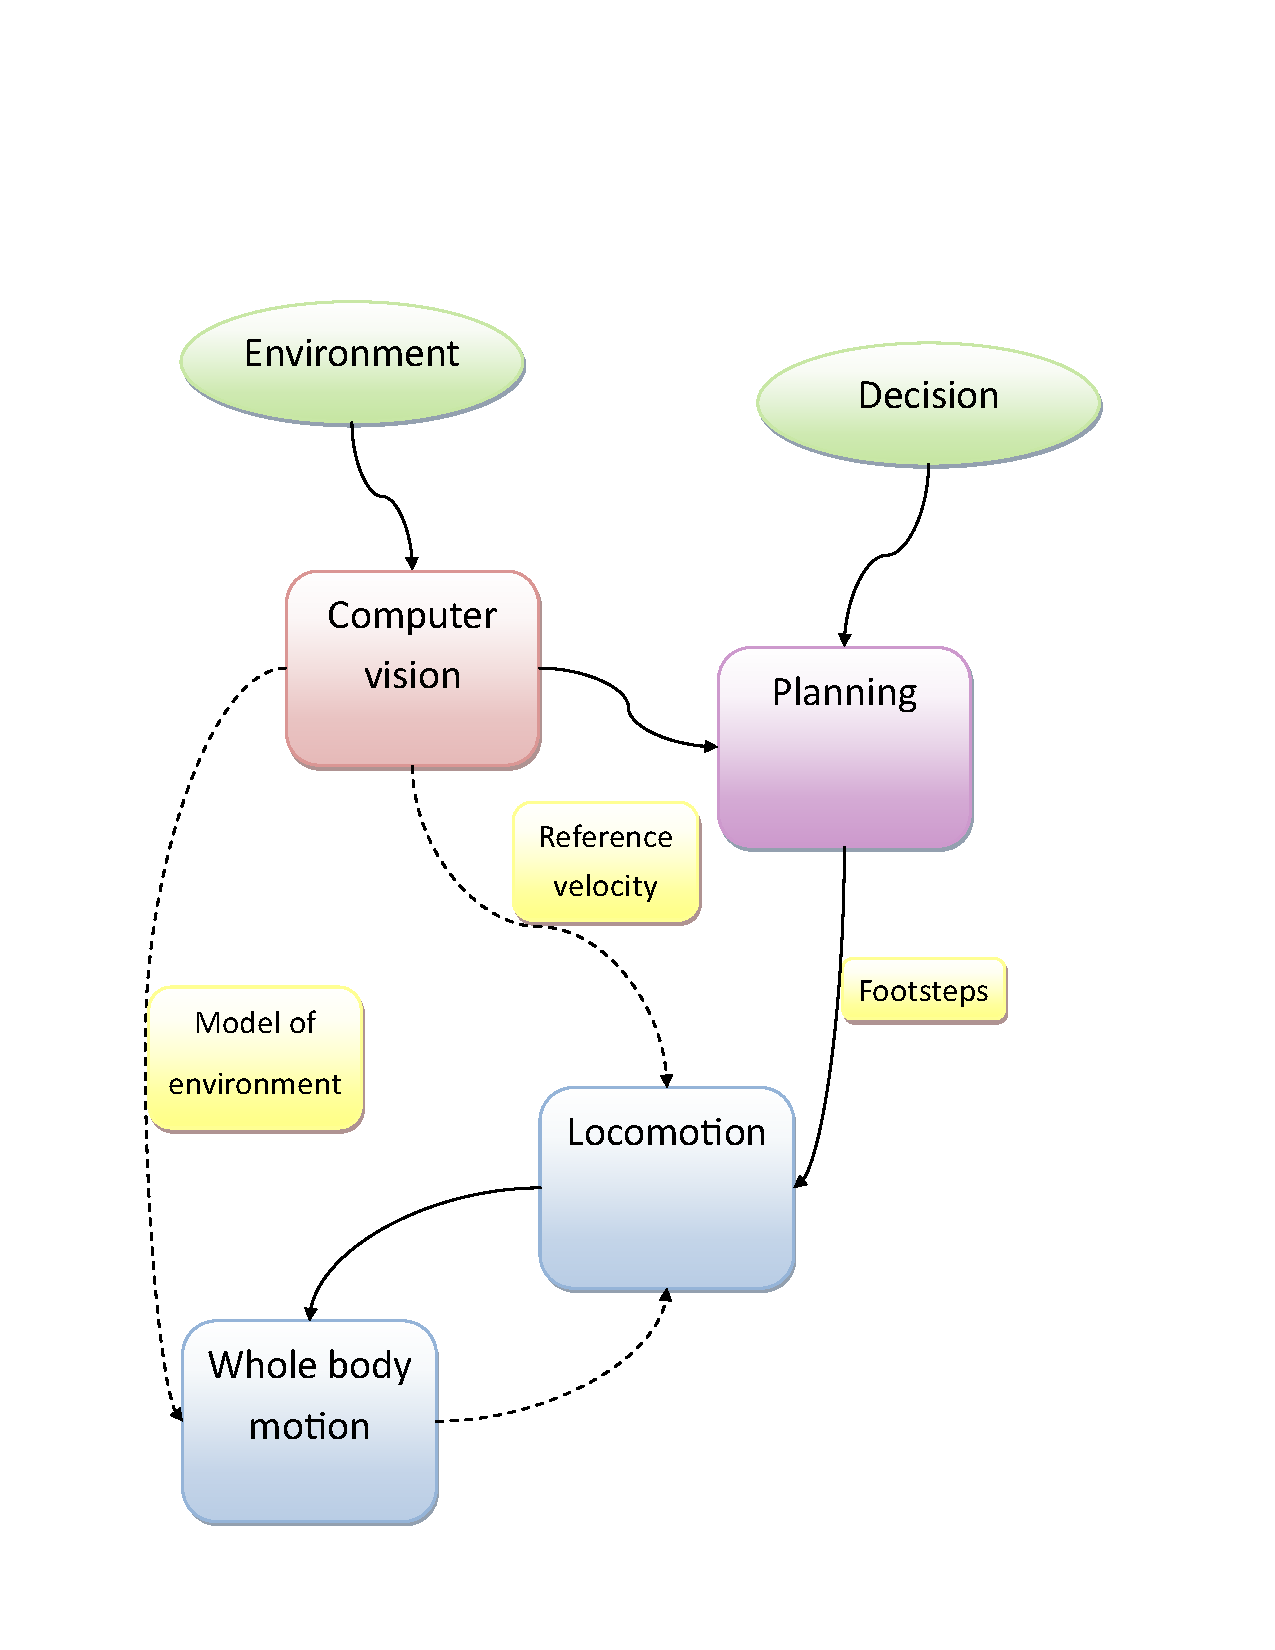
\includegraphics[scale=0.5]{figures/general-diagram.pdf}
\caption[]{ \label{Fig:GeneralDiagram} Workflow of a humanoid robot executing motion tasks using perception.}
\end{figure}

In this thesis we address the problem of the link between vision and motion generation. Building upon the work of several authors throw the years, our main contributions are,

\begin{itemize}
\item The fully integration of a visual servoing scheme within the walking motion generation using Linear Model Predictive Control (MPC);
\item The filling of the gap between traditional motion planning approaches and on-line locomotion generation algorithms;
\item The providing of 3D models of the escene in front of the robot to be used by an inverse-dynamics based approach to walk on rough terrain;
\item And finally, the validation in simulation of the proposals.
\end{itemize}

The rest of this manuscript is organized as follows. In chapter \ref{Chap:Related-Work} we state the problem and briefly recall the work that has been done on it. In chapter \ref{Chap:Visual-Servoing} We present an approach to introduce visual information in the walking pattern generator for humanoid robots. We make use of visual servoing withmodel predictive control (MPC), which is joined to the walking motion generator. Since visual servoing with MPC is a nonlinear optimization problem, we propose a linearization scheme in order to keep it as a Quadratic Program (QP) and introduce it within the pattern generator. In chapter \ref{Chap:Visual-Planning} we propose a method for reactive walking allowing visual servoing and adaptation of footsteps trajectories in real-time. This is done by building upon recent advances in the fields of optimal control for a walking pattern generator~\citep{HerdtAR2010} and planning for a nonholomic robot with field-of-view constraints ~\citep{Salaris:2010}. In chapter \ref{Chap:3DReconstruction} we present a 3D reconstruction system of the ground in front of the robot. This model allows to an inverse dynamics control scheme to know the ground structure where the swinging foot is going to step on. Finally in chapter \ref{Chap:Conclusions} we present the final discusion and future work.




% State of the Art
%\begin{savequote}[10cm]
%{\it ``Part of the inhumanity of the computer is that, once it is competently programmed and working smoothly, it is completely honest.''}
%\qauthor{Isaac Asimov}
%\end{savequote}

\chapter{Related work} 
\label{Chap:Related-Work}

Recently, very efficient control systems for humanoid robots walking generation have been proposed.
They use dynamical balance criteria such as the Center Of Pressure (CoP) and may be very reactive since foot step placement can be computed online \citep{HerdtAR2010}. In this methodollogy the CoM and CoP trajectories and footstep positions are computed automatically. This result is fed to a whole-body controller to deal coherently with the three cases. Here, the notion of footsteps disappears, allowing the user to provide a reference velocity as input to the pattern generator. Moreover, because the range of footsteps is explored by a guided search in the space of the whole-body controller transitions, a large set of possible footsteps is available in real-time.

Most of these techniques are based on Linear Model Predictive Control (LMPC). LMPC previews the behavior of the system if one applies a sequence of controls and allows us to estimate the optimal control sequence for a given horizon. In the next iteration, one applies the first next optimal control. Remarkably, LMPC can be expressed as a Quadratic Program (QP), that is the minimization of quadratic errors subject to a set of constraints.
Handling explicitly the constraints in the QP is one of the main advantages of this formulation. 
Furthermore, there are very efficient techniques to solve QPs.

The next step would be to close the control loop and use sensors information as feedback, e.g. in positioning tasks. In general humanoid walking control assume that the robot foot steps are defined before computing the actual joint control to realize it. They generally follow a perception-decision-action scheme: footsteps on time horizon are defined upon sensors information on the environment, from the footsteps center of mass trajectories (CoM) are computed to respect balance constraints. Legs control is computed by inverse kinematics. This perception-decision-action loop has proven to be fast enough to realize impressive demonstrations for stair-climbing and obstacle avoidance \citep{Lorch02,Chestnutt07,Michel07,Guttmann08}. 

On the other hand, for reactive positioning tasks, visual servoing techniques have proven to be useful \citep{ChaumetteRAM2006, ChaumetteRAM2007}. Dune et al. \citep{DuneIROS2010} proposed a visual control scheme for humanoid robots using walking pattern generation as a black box. The desired velocity of the center of mass (CoM) is computed using visual servoing and it is used as a reference in the pattern generator. The main disadvantage with this approach is that the visual servoing scheme and the pattern generator are completely decoupled so the visual information is not directly feeding the pattern generator.

On the other hand, visual servoing has been successfully applied in Model Predictive Control Schemes \citep{Allibert2010}. The main problem is that the dynamics of the camera and the projection itself are nonlinear functions for which non-linear programming are required. However, this may be time consuming and hence does not fit into an online walking pattern generator.

Parallely, research has been led towards planning trajectories that are appropriate for humanoid robots walking in cluttered environments, with different types of restrictions (e.g. \citep{Chestnutt2005, jib-IJHR2010}). 
From the seminal work of \citep{Chestnutt2005}, a main trend of research in footstep planning has been to consider a limited set of known actions (quite often footsteps) and transitions, and to find an optimal path over them. The use of a fixed-set-of-actions approach can be limiting, as it may produce unnecessary motions near the obstacles \citep{Bourgeot:IROS:2002}, while not usually dealing with the problem of robust perturbation rejection. 

A vast amount of work exist to lessen the amount of movements generated around the obstacles. Chestnutt et al. proposed in \citep{Chestnutt:ICRA:2007} an adaptation mechanism to search around the set of transitions. More recently, Hornung et al. \citep{Hornung:ICRA:2012}, proposed a method to deal with highly dynamical environments by keeping both, accurate short-term goals and rough long-term goals. As doing this may lead to local optima, the author propose a method to automatically adapt the set of actions according to the environment traversability characteristics. 

Regarding the problem of robust perturbation rejection, several advances have also been done. They can be divided into three strategies: (1) ankle-foot stabilization, (2) whole-body stabilization, and (3) footstep generation. 
Using the capture-point or the Center-of-Pressure (CoP) as an indicator of stability, one can switch between a Finite-State-Machine strategy~\citep{Nishiwaki:ijrr:2009} and a learned strategy \citep{SeungJoon:ichr:2011}.

From an application point of view, however, it is very difficult to decouple planning and control from each other. Planning is needed to avoid local optima and control is needed to reject disturbances and adapt to modeling errors. Some planning methods try to account for the motion and control capabilities of the humanoid robot by using inverse kinematics \citep{kanoun:ijrr:2011}. Despite real-time implementation \citep{Dang:ichr:2011}, this method suffers from local minima in planning footsteps. As in \citep{Vahrenkamp:IROS:2009}, we propose in this paper to use a planning approach integrating a constraint given by a task (e.g. visual-servoing). However, here, we modify the walking controller in such a way to use the planner as a generator of a full vector field that provides new local solutions from any given configuration and not only as a provider of single reference trajectories.


% Visual servoing
\chapter{Visual servoing} 
\label{Chap:Visual-Servoing}


\section{Visual servoing and MPC}

\label{sec:vs}

Visual servoing aims at controlling the motion of a robot equipped with a camera, by minimizing errors between observed features and their corresponding reference features. The nature of the features differentiates schemes of visual servoing: Image based visual servoing (IBVS) uses only image features; Position based visual servoing (PBVS) uses the 3-D pose(s) of object(s) of interest. In any of these cases of feedback, one may use a velocity controller such as

$$
\text{v}^c = -\lambda L_e^{+}e,
$$

where $e$ is the vector of errors, $\text{v}^c$ is the velocity of the camera and $L_e^{+}$ is the Moore-Penrose pseudo-inverse of the interaction matrix $L_e$, that is, the matrix relating the velocity of the features and the velocity of the camera.

Now, in walking pattern generation (see Section~\ref{sec:wpg}), MPC is used to estimate a sequence of optimal controls at some horizon, because of the step-based nature of walking. Hence, we want to orient the optimization of the foot placement by taking into account the expected evolution of the visual servoing (VS) errors so that, instead of minimizing the VS errors at current time $k$, one would like to foresee its evolution at some horizon $[k+1,k+N]$. 

In~\cite{Allibert2010}, such a time horizon-aware scheme has been proposed. The visual predictive control (VPC) is introduced as:

\begin{eqnarray}
\label{Eq:MinVisualFeatures}
 \min_{U_{k}} \;&& \sum\limits_{j=k+1}^{k+N} [s^d_j - s^m_j]^{\transpose} W_j [s^d_j - s^m_j], \\
 \mbox{subject to} \; && s^d_j = s^{*}_j - \epsilon_j, \\
 \label{Eq:ConstraintDynamicModel}
 && q_j = f(q_{j-1},u_{j-1}), \\
 \label{Eq:ConstraintProjection}
 && s^m_j = h(q_j).
\end{eqnarray}

In Eq.~\ref{Eq:MinVisualFeatures}, $U_{k}=u_{k:k+N-1}$ are the series of controls to be applied, $q_j$ is the state, and $s^*_j$, $s^d_j$ and $s^m_j$ are respectively the reference, desired and predicted positions of the visual features. The terms $\epsilon_j$ are the errors $s_j-s^m_j$ between real and predicted feature positions.
Allibert et al. assume $\epsilon_j$ constant over the prediction horizon, equal to $\epsilon_k=s_k-s^m_k$, i. e. the error at current time $k$, because by definition the $s_j$ are not known for $j>k$.
Since our landmarks are static, $s^*_j \stackrel{\mbox{\tiny def}}{=} s^*$, and since the prediction errors are constant on the horizon window, $s^d_j=s^d_k=s^*-\epsilon_k$ are constant in the prediction horizon.

Eq.~\ref{Eq:ConstraintDynamicModel} is the dynamic model, that estimates the new state given the last state/control pair. In general, this function is non-linear. We will see how to deal with this non-linearity.

Eq.~\ref{Eq:ConstraintProjection} is also a non-linear function that estimates the output of the model $s^m_j$, given the current state $q_j$. This equation implements the pinhole camera projection model.

Matrix $W_j$ in Eq.~\ref{Eq:MinVisualFeatures} is a positive definite matrix  used to weight errors in the prediction horizon. As suggested in~\cite{Allibert2010}, we   consider equal weights for all features errors, $W_j = diag(w_j)$. 

Here, $s^m_j$ is the collection of all the predicted features at time $j$, that is, for $M$ features $s^m_j = ( s_{1,j}^m, s_{2,j}^m, \hdots, s_{M,j}^m )^{\transpose} $. Eq.~\ref{Eq:MinVisualFeatures} can be rewritten as

\begin{equation}
\label{Eq:MinVisualFeatures2}
 \min_{U_{k}} \; \sum\limits_{l=0}^{M}  [S^d_{l} - S^m_{l,k}]^{\transpose} W [S^d_{l} - S^m_{l,k}],
\end{equation}

with $S^m_{l,k}$ stacking the features positions in the horizon: $S^m_{l,k} =  \left(
  s^m_{l,k+1},
  s^m_{l,k+2},
 \dots,
  s^m_{l,k+N}
 \right)^{\transpose}$, $S^d_{l}$ stacking the corresponding desired positions, and $W = diag(w_{k+1},w_{k+2},...,w_{k+N})$.

\section{Walking pattern generation}

\label{sec:wpg}

Most of the current walking motion generation schemes for humanoid robots are based on the model proposed in~\cite{Kajita2003}, that focuses in the trajectory of the center of mass to generate balanced and stable motions. If we suppose that the trajectory has periodic piece-wise constant jerks on a time interval $T$, we can express the CoM dynamics on the $x$-axis as

$$
\left\{
\begin{array}{ccc}
 \hat{x}_{k+1} &=& A \hat{x}_k + B \dddot{x}_k\\
 \xi^x_{k} &=& C \hat{x}_k 
\end{array}
\right.
$$

where $\hat{x}_{k} = \left( x_k, \dot{x}_k, \ddot{x}_k \right)^{\transpose}$ stacks the $x-$position, 
velocity and acceleration of the robot CoM at time $k$, and

\begin{equation*}
A = \left(
\begin{matrix}
1 & T & T^2/2 \\
0 & 1 & T \\
0 & 0 & 1
\end{matrix}
\right) \text{, }
B = \left(
\begin{matrix}
T^3/6 \\
T^2/2 \\
T
\end{matrix}
\right) \text{ and }
C = \left(
\begin{matrix}
1 \; 0 \; \frac{c_z}{g} \\
\end{matrix}
\right)
\end{equation*}

and ${\xi}^x_k$ is the CoP at time $k$.
By applying recursively the dynamics, we can express the trajectory of the CoM in terms of the initial position $\hat{x}_k$ and the sequence of jerks $\dddot{X}_k = (\dddot{x}_k, \dddot{x}_{k+1},...,\dddot{x}_{k+N-1})^{\transpose}$,

\begin{equation}
 \label{Eq:PosCMHorizon}
 X_{k+1} = \left(
 \begin{matrix}
  x_{k+1} \\
  \vdots \\
  x_{k+N}
 \end{matrix}
 \right) = P_{ps} \hat{x}_k + P_{pu} \dddot{X}_k.
\end{equation}

Similar expressions can be obtained for the velocity and acceleration of the CoM, and for the $y$ component.

In the original approach~\cite{Kajita2003}, the positions of the center of pressure (CoP) must be predefined, so preliminary footstep planning was necessary. Later on, an interesting re-formulation was proposed to handle automatic footstep placement~\cite{HerdtAR2010}. This approach makes use of a reference velocity $(\dot{X}_{k+1}^{ref},\dot{Y}_{k+1}^{ref})$ and the resulting constrained optimization problem is:

{\scriptsize
\begin{eqnarray}
\label{Eq:MinJerk}
\nonumber
 \underset{U_{k}}{\min} \; && \dfrac{\alpha}{2} \left\| \dddot{X}_k \right\|^2 + \dfrac{\beta}{2} \left\| \dot{X}_{k+1} - \dot{X}_{k+1}^{ref} \right\|
 + \dfrac{\gamma}{2} \left\| Z_{k+1}^x - Z_{k+1}^{x_{ref}} \right\| \\
 && + \dfrac{\alpha}{2} \left\| \dddot{Y}_k \right\|^2 + \dfrac{\beta}{2} \left\| \dot{Y}_{k+1} - \dot{Y}_{k+1}^{ref} \right\|
 + \dfrac{\gamma}{2} \left\| Z_{k+1}^y - Z_{k+1}^{y_{ref}} \right\|,
\end{eqnarray}
}
with $U_{k} \stackrel{\mbox{\tiny def}}{=}  \left( \dddot{X}^{\transpose}_k, (X_k^f)^{\transpose}, \dddot{Y}^{\transpose}_k, (Y_k^f)^{\transpose} \right)^{\transpose}$, and
 $X^f_k, Y^f_k$ are the footsteps positions, now taken as additional variables. 
We also define the vector of CoP values on the horizon as $Z_{k+1}^x = [ {\xi}^x_{k+1} \; \cdots \; {\xi}^x_{k+N}]$. 
The reference values $Z_{k+1}^{x_{ref}}$ are the center of the support polygon at each iteration.
This can be written as a canonical Quadratic Program (QP) 

\begin{equation*}
 \underset{U_k}{\min} \; \dfrac{1}{2} U_k^{\transpose} Q_k U_k + p_k^{\transpose} U_k.
\end{equation*}

The objective of our approach and the main contribution of this paper is that instead of controlling the robot through the references velocities, it is realized using visual features. At the end, our approach summarizes in replacing the reference velocities in Eq. \ref{Eq:MinJerk} by Eq. \ref{Eq:MinVisualFeatures2}. We would also want to keep the problem as a QP so it can be solved efficiently in real time.

\section{Integrating the visual servoing to the walking motion generator}
\label{sec:integration}
If we introduce directly Eq. \ref{Eq:MinVisualFeatures2} in Eq. \ref{Eq:MinJerk}, we will not have a QP anymore due to the non-linear constraints, namely Eqs. \ref{Eq:ConstraintDynamicModel} and \ref{Eq:ConstraintProjection}. We can directly solve the first problem (Eq. \ref{Eq:ConstraintDynamicModel}) by using the dynamic model in Eq. \ref{Eq:PosCMHorizon}. In this case there is no rotation, but we will see that we can introduce it in a decoupled way without losing the QP formulation.

\subsection{Linearization of the observation model}

As we said, Eq. \ref{Eq:ConstraintProjection} implements the pinhole camera model. Let $p^{w}_{l'} = [x^{w}_{l'},y^{w}_{l'},z^{w}_{l'}]^{\transpose}$ be the position of the {l'}-th landmark in the world reference frame. At time $j$, one can compute the projection to the image plane by first transforming the landmark position to the camera frame with the homogeneous transform $T^{mc} T^{wm}_j$ and then applying the projection,

\begin{equation}
\label{Eq:Projection}
\begin{array}{c}
 \left(
 \begin{matrix}
  u_{l',j} \\
  v_{l',j}
\end{matrix}
\right)
  =
 \left(
 \begin{matrix}
  u(x^{c}_{l',j},y^{c}_{l',j},z^{c}_{l',j}) \\
  v(x^{c}_{l',j},y^{c}_{l',j},z^{c}_{l',j})
 \end{matrix}
 \right)
 =  \left(
 \begin{matrix}
  x^{c}_{l',j} / z^{c}_{l',j}\\
  y^{c}_{l',j} / z^{c}_{l',j}
 \end{matrix}
 \right),
 \end{array}
\end{equation}

where $T^{wm}_j$ is the transformation from the world frame to the CoM frame and $T^{mc}$ is the transformation from the CoM frame to the camera frame, which is not variable in our approach. Note that

{\small
$$
T^{wm}_j = (T^{mw}_j)^{-1} = 
\left(
\begin{matrix}
(R^{mw}_j)^{-1} & -(R^{mw}_j)^{-1}t^{mw}_j \\
0_{1 \times 3} & 1
\end{matrix}
\right)
$$ 
}

where $t^{mw}_j$ is the position of the CoM in the world frame at time $j$, which depends in our control variables through Eq. \ref{Eq:PosCMHorizon}.
$R^{mw}_j$ is the direction of the robot waist according to the world reference frame at time $j$. In our current formulation 
there is no free variables modifying this quantity, because it would make the problem non-linear. More details
about this problem are given in Section~\ref{subsection:control_of_the_rotation_angle}.

If we use directly Eq. \ref{Eq:Projection} (non-linear), we will lose the QP formulation. 
We know that Eq.~\ref{Eq:Projection} is a projection $h:\mathbb{R}^3 \rightarrow \mathbb{R}^2$.

\begin{equation*}
%\label{Eq:ProjectionTaylor}
h(x,y,z) =
 \left(
 \begin{matrix}
  u(x,y,z) \\
  v(x,y,z)
 \end{matrix}
 \right)
 = \left(
 \begin{matrix}
  x / z\\
  y / z
 \end{matrix}
 \right).
\end{equation*}


We know also from MPC that prediction is done over a finite horizon. So it might be enough to use a first order approximation of $h$ for small $(dx,dy,dz)$ so that we can maintain the QP form.

Now, by using a Taylor series for $u(x,y,z)$ around some point $(x_0,y_0,z_0)$ and substituting the derivatives,

%$$
%\begin{array}{c}
% u(x_0+dx,y_0+dy,z_0+dz) = u(x_0,y_0,z_0) +\\
% u_x(x_0,y_0,z_0)dx + u_y(x_0,y_0,z_0)dy + \\
% u_z(x_0,y_0,z_0)dz + \mathcal{O}(dx,dy,dz)^2
%\end{array}
%$$

$$
\left\{
\begin{array}{c}
%\label{Eq:ProjectionTaylorApproxU}
\nonumber
 u(x_0+dx,y_0+dy,z_0+dz) \approx \frac{x_0}{z_0} +  \frac{dx}{z_0} - \frac{x_0 dz}{z_0^2},\\
 v(x_0+dx,y_0+dy,z_0+dz) \approx \frac{y_0}{z_0} +  \frac{dy}{z_0} - \frac{y_0 dz}{z_0^2}.
\end{array}
\right.,
$$

with $dx=x-x_0$, $dy=y-y_0$ and $dz=z-z_0$. 

We propose to apply such a linearization of Eq.~\ref{Eq:Projection} for the whole horizon, around the first position $(j=k)$ of landmark $l'$, i.e. at the linearization point $(x^{c}_{l',k},y^{c}_{l',k},z^{c}_{l',k})$. 

This way, we can express the predicted position of the landmark $l'$ linearly at time $j>k$ in the horizon:

\begin{equation*}
%\label{Eq:ProjectionLinearized}
 \left(
 \begin{matrix}
  u_{l',j} \\
  v_{l',j}
 \end{matrix}
 \right)
 = \left(
 \begin{matrix}
  \pi^{11}_{l',k} x^{c}_{l',j} + \pi^{13}_{l',k} z^{c}_{l',j}+ u_{l',k}\\
  \pi^{22}_{l',k} y^{c}_{l',j} + \pi^{23}_{l',k} z^{c}_{l',j} + v_{l',k}
 \end{matrix}
 \right),
\end{equation*}

where $u_{l',k} = x^{c}_{l',k} / z^{c}_{l',k}$ and $v_{l',k} = y^{c}_{l',k} / z^{c}_{l',k}$ are the initial positions of the landmarks in the horizon and the coefficients $\pi_{ij}$ the elements of the matrix

\begin{equation*}
\Pi_{l',k} = \left(
\begin{matrix}
 1/z^{c}_{l',k} & 0 & - u_{l',k} / z^{c}_{l',k} \\
 0 & 1/z^{c}_{l',k} & - v_{l',k} / z^{c}_{l',k}
\end{matrix}
\right),
\end{equation*}

which is the classical definition of the interaction matrix in Image-Based Visual Servoing.

Finally, we can express the projection of the $l'-th$ landmark (constraint \ref{Eq:ConstraintProjection}) as :

\begin{equation}
\label{Eq:Features}
 \left(
 \begin{matrix}
  u_{l',j} \\
  v_{l',j}
 \end{matrix}
 \right) = 
\left[
\begin{array}{cc}
\multirow{2}{*}{$\Pi_{l',k}$} & u_{l',k} \\
& v_{l',k} \\
\end{array}
\right]
 T^{mc} T^{wm}_j \left( \begin{array}{c}
 p^{w}_{l'}\\
 1
 \end{array}\right),
\end{equation}

so that we can now introduce the visual features in the pattern generator. Expanding terms in Eq.~\ref{Eq:Features} for the first row and setting $\Pi^u_{l',k}$ as the first row of matrix $\Pi_{l',k}$,

\begin{eqnarray}
\label{Eq:FeatExpanded}
 u_{l',j} &= &\Pi^u_{l',k} (R^{wc} p^{w}_{l'} + R^{wc} t^{mw}_j + t^{mc}) + u_{l',k}.
\end{eqnarray}

Since $R^{wc} t^{mw}_j = R^{wc}_1 x_j + R^{wc}_2 y_j + R^{wc}_3 z_j$, where $R^{wc}_i$ is the $i$-th column of $R^{wc}$
\footnote{To simplify the notations $R^{wc}=R^{mc}R_j^{wm}$}
and $x_j,y_j,z_j$ the position of the CoM at time $j$ (see Section~\ref{sec:wpg}). We can rewrite Eq.~\ref{Eq:FeatExpanded}

\begin{equation}
\label{Eq:FeaturesUReduced}
 u_{l',j} = a^u_{l',k} x_j + b^u_{l',k} y_j + c^u_{l',k},
\end{equation}

with 
$$
\left\{
\begin{array}{ccl}
a^u_{l',k} & = & \Pi^u_{l',k} R^{wc}_1\\
b^u_{l',k} & = & \Pi^u_{l',k} R^{wc}_2\\
c^u_{l',k} & = & \Pi^u_{l',k} (R^{wc} p^{w}_{l'} + t^{mc} + R^{wc}_3 z_j) + u_{l',k}.
\end{array}
\right.
$$
Equivalently,

\begin{equation}
\label{Eq:FeaturesVReduced}
  v_{l',j} = a^v_{l',k} x_j + b^v_{l',k} y_j + c^v_{l',k}.
\end{equation}

Stacking the features $u_{l',j}$ and the CoM positions for the whole horizon and using Eq.~\ref{Eq:PosCMHorizon}, we get a vector $S^m_{l,k}$ similar to the one introduced in Eq.~\ref{Eq:MinVisualFeatures2} 

\begin{equation*}
S^m_{l',k} = A^u_{l',k} X_{k+1} + B^u_{l',k} Y_{k+1} + C_{l',k}^u,
\end{equation*}

with 
$$
\begin{array}{ccl}
A^u_{l',k} &=& a^u_{l',k} I_{N\times N}\\
B^u_{l',k} &=& b^u_{l',k} I_{N\times N}\\
C_{l',k}^u &=& c^u_{l',k} (1,1,...,1)^{\transpose}
\end{array}
$$

 which corresponds to the predicted coordinates $u$ of the landmark $l'$-th in the horizon.
The equivalent equations for the $v$ coordinates of the same landmark are straightforward.

Every projected landmark provides two coordinates $(u,v)$ and we treat each one as an individual feature. This means that the $l$-th feature is the $u$ coordinate in the image of the landmark $l' = \left \lfloor l/2 \right \rfloor$ for $l$ even, and the $v$ coordinate for $l$ odd.

Generalizing to all features, we have:
\begin{equation}
\label{Eq:FeaturesStacked}
 S^m_{l,k} = A_{l,k} X_{k+1} + B_{l,k} Y_{k+1} + C_{l,k},
\end{equation}

with $A_{l,k} = A^u_{l',k}$ for $l$ even and $A_{l,k} = A^v_{l',k}$ for $l$ odd. The same holds for $B_{l,k}$ and $C_{l,k}$.

Finally, we can introduce visual servoing in the walking generation with the QP:

\begin{eqnarray*}
\nonumber
 \min_{U_k} \; && \dfrac{\alpha}{2} \left\| \dddot{X}_k \right\|^2
 + \dfrac{\gamma}{2} \left\| Z_{k+1}^x - Z_{k+1}^{x_{ref}} \right\| \\
 \nonumber
 && + \dfrac{\alpha}{2} \left\| \dddot{Y}_k \right\|^2
 + \dfrac{\gamma}{2} \left\| Z_{k+1}^y - Z_{k+1}^{y_{ref}} \right\| \\
 \nonumber
 && + \dfrac{\beta}{2} \sum\limits_{l=0}^{M}  [S^d_{l}- S^m_{l,k}]^{\transpose} W [S^d_{l} - S^m_{l,k}],
\end{eqnarray*}

and as a canonical QP:
{\small
\begin{equation*}
\underset{U_k}{\min} \; \dfrac{1}{2} U_k^{\transpose} Q_k U_k + p_k^{\transpose} U_k
\end{equation*}
}
{\small
\text{ with }
\begin{equation*}
Q_k = \left( \begin{array}{cc}
Q_k' & 0 \\
0 & Q_k'
\end{array}
 \right) + \hat{Q}_k,
\end{equation*}
}

{\scriptsize
\begin{equation*}
 Q_k' = \left(
 \begin{array}{cc}
 \alpha I + \gamma P^{\transpose}_{zu}P_{zu} & - \gamma P^{\transpose}_{zu}V_{k+1} \\
 -\gamma V^{\transpose}_{k+1} P_{zu} & \gamma V^{\transpose}_{k+1} V_{k+1}
 \end{array}
 \right),
\end{equation*}
}

{\scriptsize
\begin{equation*}
 \hat{Q}_k = \left(
 \begin{matrix}
 \beta \sum\limits_l P_{pu}^{\transpose} A_{l,k}^{\transpose} {W} A_{l,k} P_{pu} & 0 & \beta \sum\limits_l P_{pu}^{\transpose} A_{l,k}^{\transpose} {W} B_{l,k} P_{pu} & 0\\
 0 & 0 & 0 & 0 \\
 \beta \sum\limits_l P_{pu}^{\transpose} B_{l,k}^{\transpose} {W} A_{l,k} P_{pu} & 0 & \beta \sum\limits_l P_{pu}^{\transpose} B_{l,k}^{\transpose} {W} B_{l,k} P_{pu} & 0 \\
 0 & 0 & 0 & 0
 \end{matrix}
 \right)
\end{equation*}
}

and $p_k = p_k' + \hat{p}_k$,

{\scriptsize
\begin{equation*}
 p'_k = 
 \left(
 \begin{array}{c}
 \gamma P^{\transpose}_{zu}(P_{zs} \hat{x}_k - V_{k+1}^c X_k^{fc}) \\
 -\gamma V^{\transpose}_{k+1}(P_{zs}\hat{x}_k - V_{k+1}^c X_k^{fc}) \\
 \gamma P^{\transpose}_{zu}(P_{zs} \hat{y}_k - V_{k+1}^c Y_k^{fc}) \\
 -\gamma V^{\transpose}_{k+1}(P_{zs}\hat{y}_k - V_{k+1}^c Y_k^{fc})
 \end{array}
 \right),
\end{equation*}
}

{\scriptsize
\begin{equation*}
 \hat{p}_k = 
 \left(
 \begin{matrix}
 \beta  \sum\limits_l P_{pu}^{\transpose} A_{l,k}^{\transpose} W [A_{l,k} P_{ps} \hat{x}_k + B_{l,k} P_{ps} \hat{y}_k + C_{l,k} - S^d_l]\\
 0 \\
 \beta  \sum\limits_l P_{pu}^{\transpose} B_{l,k}^{\transpose} W [A_{l,k} P_{ps} \hat{x}_k + B_{l,k} P_{ps} \hat{y}_k + C_{l,k} - S^d_l ]\\
 0
 \end{matrix}
 \right).
\end{equation*}
}

For details on matrices $P_{ps}$, $P_{zs}$, $P_{pu}$, $P_{zu}$, $V_{k+1}$ and $V_{k+1}^c$ see~\cite{HerdtAR2010}.

\subsection{Control of the rotation angle}
\label{subsection:control_of_the_rotation_angle}
So far, we have proposed a scheme to control the trajectory of the center of mass in the $xy$ plane. However, introducing the rotation angle in the minimization problem is not straightforward without losing linearity. Furthermore, the rotation angle plays a very important role here since sometimes most of the error between $s^d$ and $s^m$ may be due to the angle between the robot and the features.

An extension of the original LMPC scheme with automatic footstep placement that deals with a reference angular velocity has been proposed in~\cite{HerdtIROS2010}. The approach is a decoupled solution, that is, it estimates first the optimal rotation angles and afterwards introduces these values as known in the main QP ($R^{mw}_j$).  This scheme should not affect the stability of the walking since inertial effects are not taken into account.

%\textbf{\small JBH: Which one is used ? Do you compare the 2 in the experiments?}

The same decoupled solution can be used in our approach. However, we propose here to apply a decoupled angle controller using a simple PID controller.
%% The following sentence is a bit redundant ?
This scheme can be replaced by the one proposed in \cite{HerdtIROS2010}.

\subsection{Visual constraints}
The introduction of visual constraints can be done by using Eq.~\ref{Eq:FeaturesUReduced} and Eq.~\ref{Eq:FeaturesVReduced}.
Any linear constraint in the image plane $(u,v)$, can be expressed as a linear constraint in the variables $U_k$.
Furthermore a convex polytope can be expressed under a linear form.
%\begin{equation}
%\label{Eq:VSConstraints}
% A 
% \left(
% \begin{matrix}
% a^u_{l',k} X_j + b^u_{l',k} Y_j + c^u_{l',k} \\
% a^v_{l',k} X_j + b^v_{l',k} Y_j + c^v_{l',k}
% \end{matrix}
% \right) \leq b.
%\end{equation}
%
It means that we can have time- and landmark-varying constraints. Commonly we only want all landmarks to follow trajectories inside of some convex polytope. Hence, constraints become constant in time and for all landmarks. This can be written as

\begin{equation}
 A'
 \left(
 \begin{matrix}
 A^u_{l',k} X_{k+1} + B^u_{l',k} Y_{k+1} + C^u_{l',k} \\
 A^v_{l',k} X_{k+1} + B^v_{l',k} Y_{k+1} + C^v_{l',k}
 \end{matrix}
 \right) \leq b',
 \text { then }
 A'' U_k \leq b''.
 \label{Eq:VSConstraintsOptimVar} 
\end{equation}

Bound constraints in the $(u,v)$ coordinates like visibility constraints are easily expressed in terms of Eq.~\ref{Eq:VSConstraintsOptimVar} and are introduced directly in the QP.

\section{Simulation results}

\label{sec:results}

We tested our approach in a simulated environment with the NAO robot model and we comment the results hereafter. We assume that no noise or modeling errors have been introduced. For all the tests, the initial position is $(0,0)$ and the desired features are set in the position $(2,1)$. First, we try without rotation, so that the robot has just to control the $x$ and $y$ velocities, which are the variables in the QP. Depending of the weights of the QP we obtain different trajectories, such as in Figs.~\ref{Fig:Results1} and \ref{Fig:Results2}. The difference between these two simulations is that we increased the $\beta $ parameter ($\beta=10^{-5}$ in the first, $\beta =10^{-4}$ in the second). The result is that the robot minimizes first the features errors, disregarding the jerks, which produces high velocities.

%% Needs more descriptions of the figures. Ex: what are the two curves in 1.c ?

\begin{figure*}[ht]
 \centering
  \subfigure[]{
 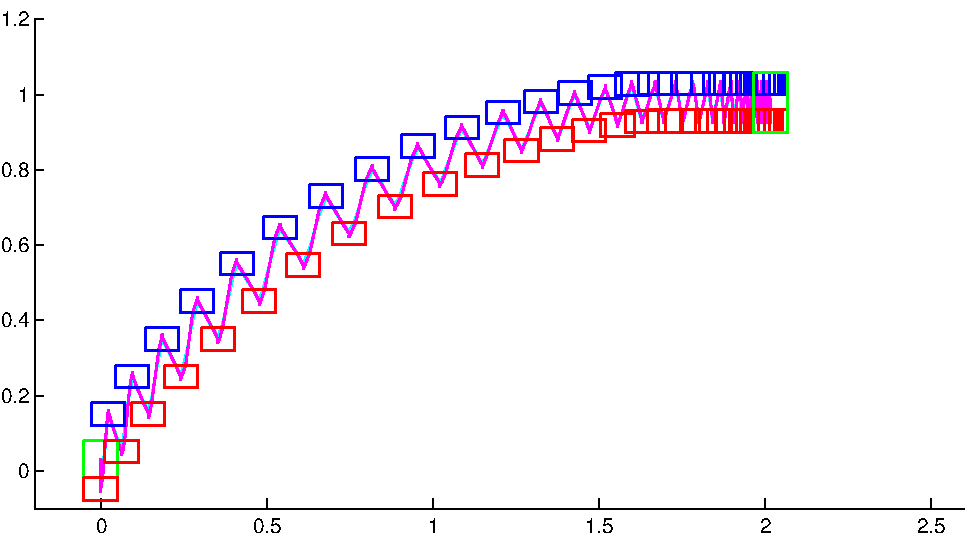
\includegraphics[scale=.46]{figures/steps1.pdf}
 \label{Fig:Results1a}
 }
 \subfigure[]{
 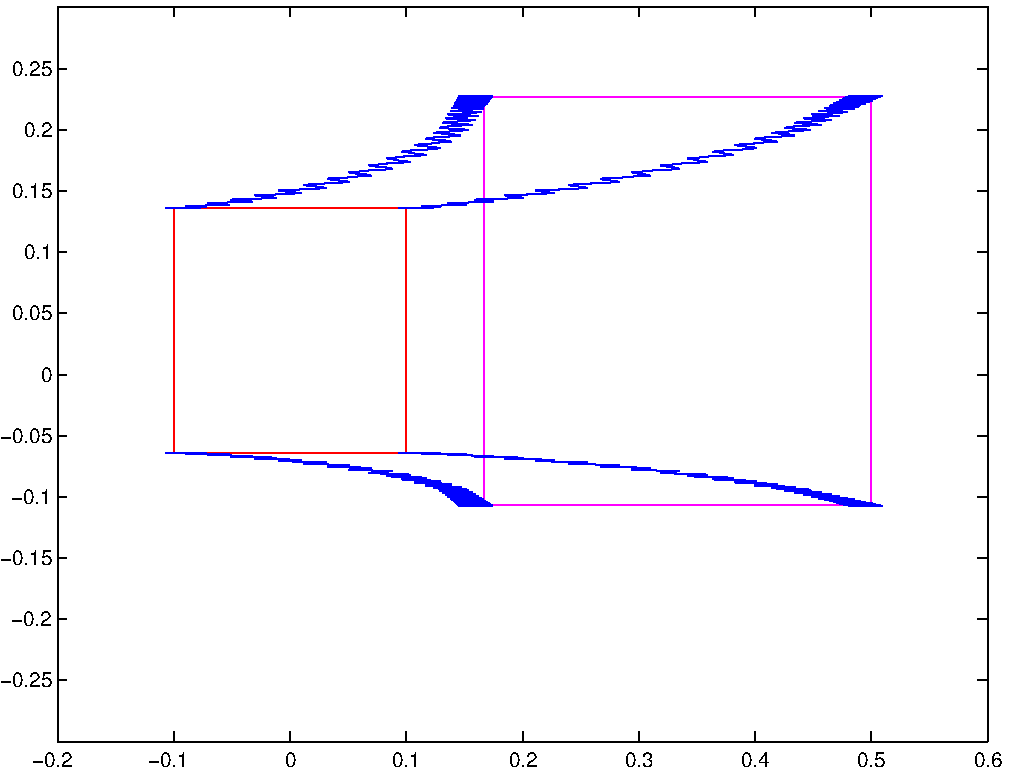
\includegraphics[scale=.27]{figures/features1.pdf}
 \label{Fig:Results1b}
 }
 \subfigure[]{
 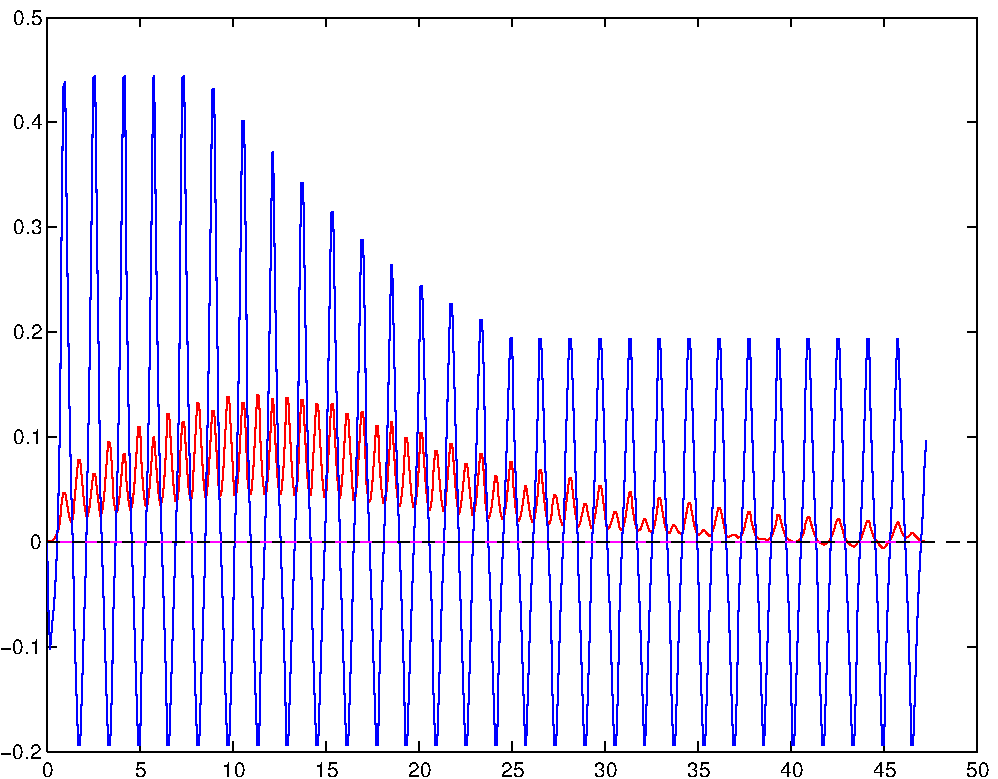
\includegraphics[scale=.27]{figures/velocities1.pdf}
 \label{Fig:Results1c}
 }
 \caption[]{\label{Fig:Results1}\small{In~\ref{Fig:Results1a}, we show the trajectory of the robot in the $x,y$ plane. The initial and final double stance phases appear in green. The single stance support feet appear in red (resp. blue) for the right (resp. left) foot. In pink, we depicted the CoP trajectory, which can be observed to remain safely in the support polygon, and in light blue the CoM trajectory. In \ref{Fig:Results1b}, we depict (in blue) the trajectory of the features in the image, with the initial positions in red and the desired positions in pink, for the first simulation.  Finally, the evolution of the velocities is shown in \ref{Fig:Results1c}. It is interesting to note the offset of the oscillatory velocity in $x$ and $y$ due to the features errors.}}
 \end{figure*}


\begin{figure*}[ht]
 \centering
  \subfigure[]{
 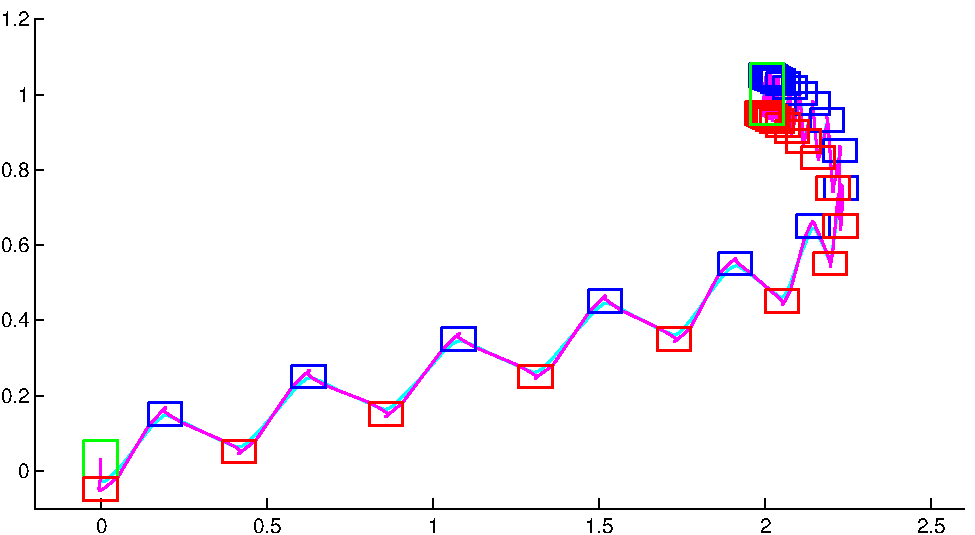
\includegraphics[scale=.46]{figures/steps2.pdf}
 \label{Fig:Results2b}
 }
 \subfigure[]{
 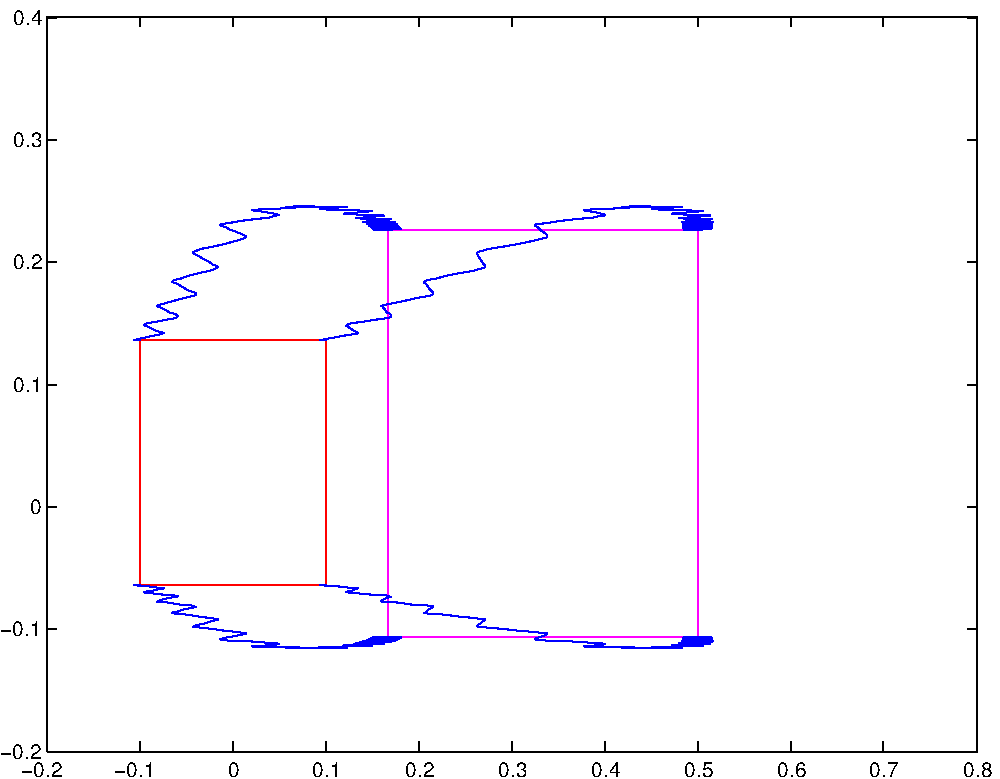
\includegraphics[scale=.27]{figures/features2.pdf}
 \label{Fig:Results2a}
 }
 \subfigure[]{
 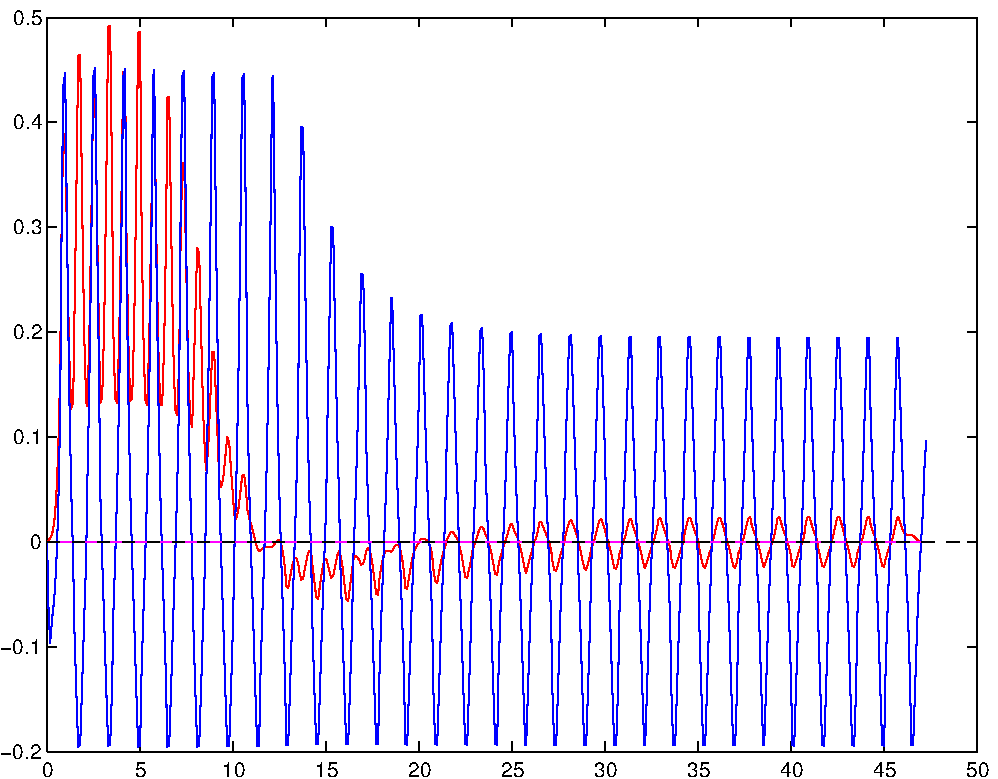
\includegraphics[scale=.27]{figures/velocities2.pdf}
 \label{Fig:Results2c}
 }
 
 \caption[]{\label{Fig:Results2}\small{The behavior of our system in the second simulation ($\beta$ is 10 times higher), with the same graphical conventions as in Fig.~\ref{Fig:Results1}. The robot is following a quite distinct trajectory, with a backwards part close to the end. As the priority is to minimize features errors, disregarding the jerks, high velocities are taken.}}
 \end{figure*}

Now we evaluate the trajectory with rotation. We recall that the rotation velocity control is decoupled from the $x$ and $y$ velocities control. It works as follows: The rotation velocity controller sets (in a decoupled way) the angular position while the main controller (QP) adapts the $x,y$ velocities in terms of this given angular position (which is known in the horizon), the visual errors, footsteps centering and jerks minimization. The results of a first simulation involving rotation is shown in Fig.~\ref{Fig:Results3}. One can observe that the dynamical balance is kept, and that most of the correction related to the rotation is done at the beginning of the trajectory. Also, in Fig.~\ref{Fig:Results4}, we can see that it is robust to perturbations: The same trajectory is followed as in Fig.~\ref{Fig:Results3} but a strong perturbation in the CoM position has been introduced, inducing peaks in the cost function and in the velocities. However, the perturbation is recovered quasi-instantly.

%  \begin{figure}[h]
%  \centering
%  \includegraphics[scale=.25]{featuresA1.png}
%  \caption[]{ \label{Fig:Image} Left image of the stereo pair.}
%  \end{figure}

\begin{figure*}[ht]
 \centering
  \subfigure[]{
 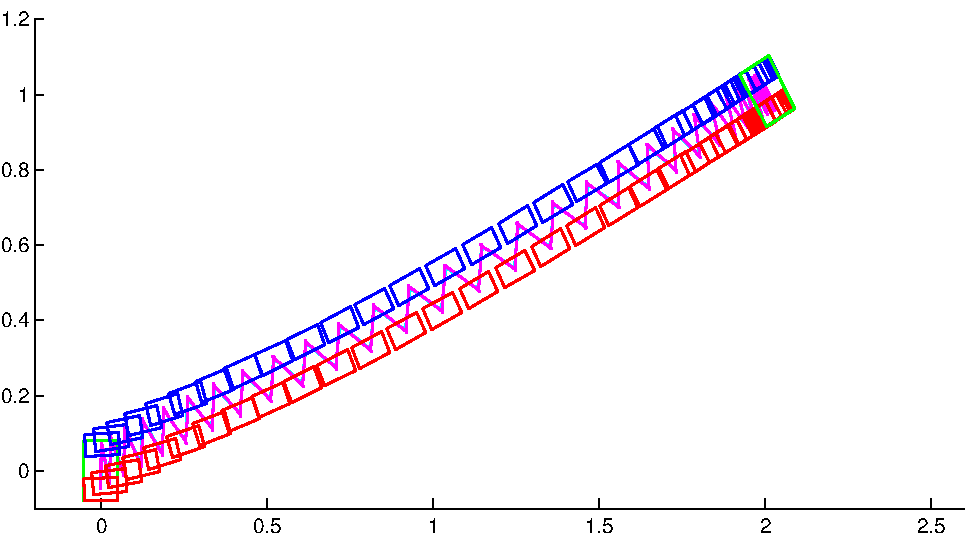
\includegraphics[scale=.46]{figures/steps3.pdf}
 \label{Fig:Results3b}
 }
 \subfigure[]{
 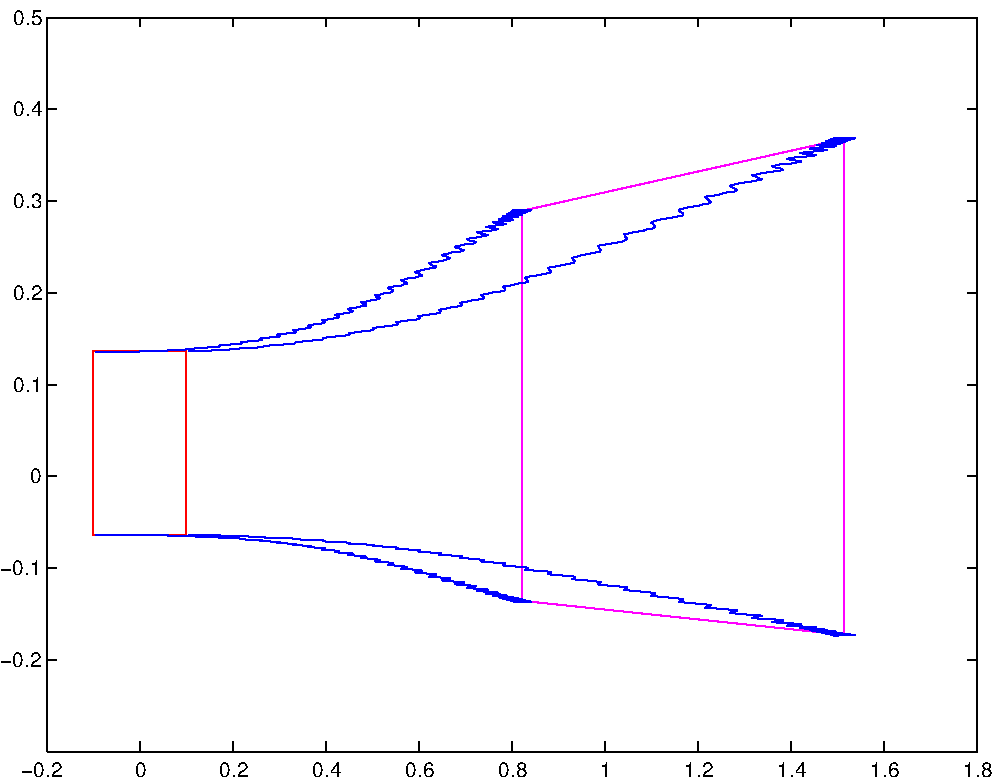
\includegraphics[scale=.27]{figures/features3.pdf}
 \label{Fig:Results3a}
 }
 \subfigure[]{
 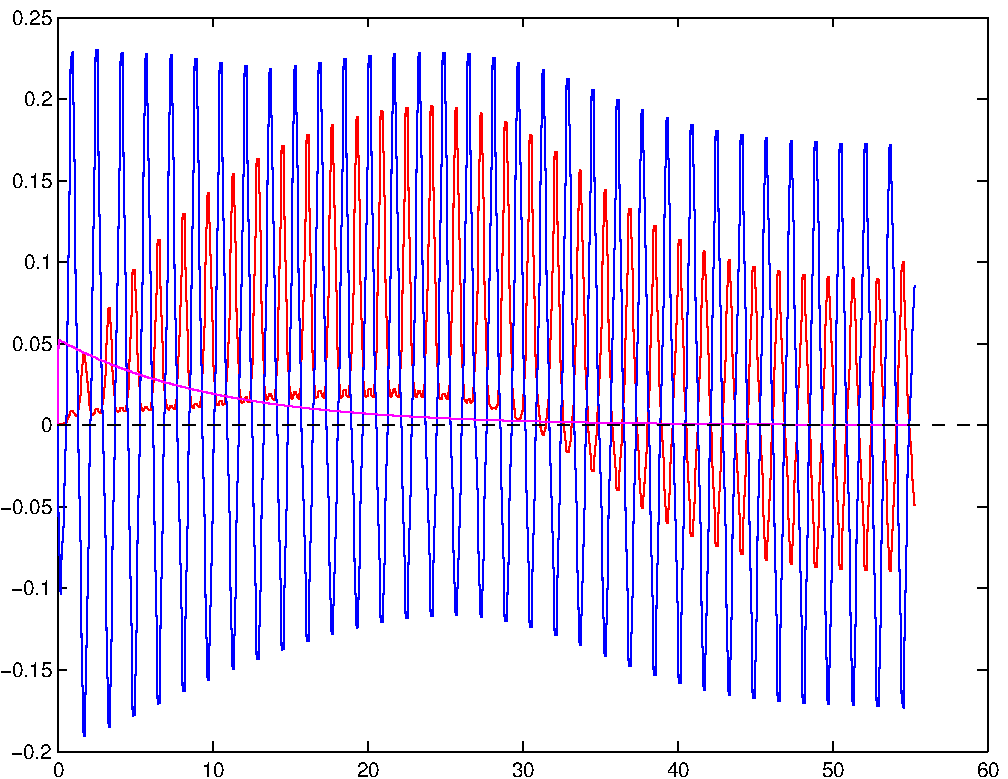
\includegraphics[scale=.27]{figures/velocities3.pdf}
 \label{Fig:Results3c}
 }
 \caption[]{\label{Fig:Results3}\small{The behavior of our system in the third simulation, involving rotation, with the same graphical conventions as in Fig.~\ref{Fig:Results1}. The robot is walking in the sagittal direction most of the time, after an initial rotation. The amplitude of the oscillation of the CoM and subsequently of the features are smaller than in the first simulation. However, we can see a non-negligible component of velocity in the positive $y$ direction, since the angle is not fully compensated. When the angle is almost fully compensated, this component disappears.}}
 \end{figure*}

\begin{figure*}[ht]
 \centering
 \subfigure[]{
 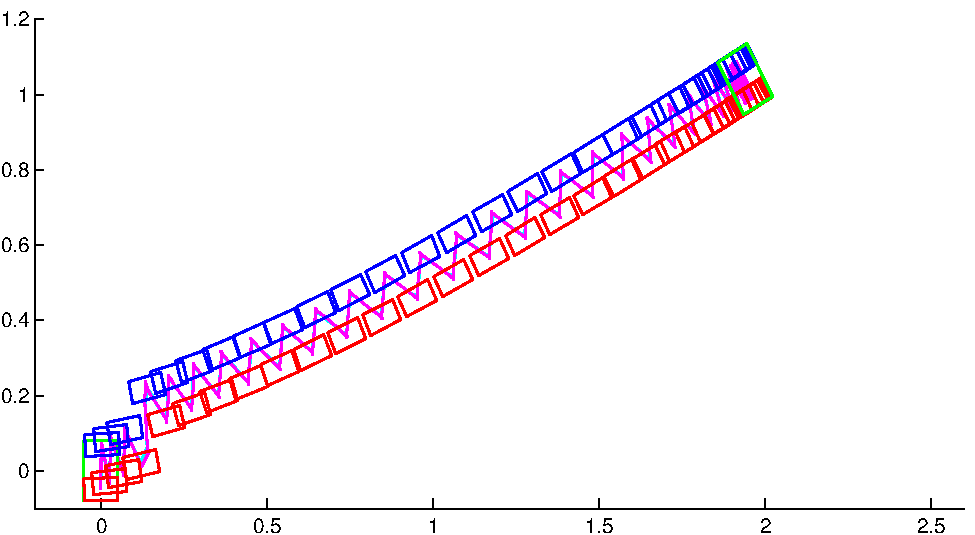
\includegraphics[scale=.46]{figures/steps4.pdf}
 \label{Fig:Results4a}
 }
  \subfigure[]{
 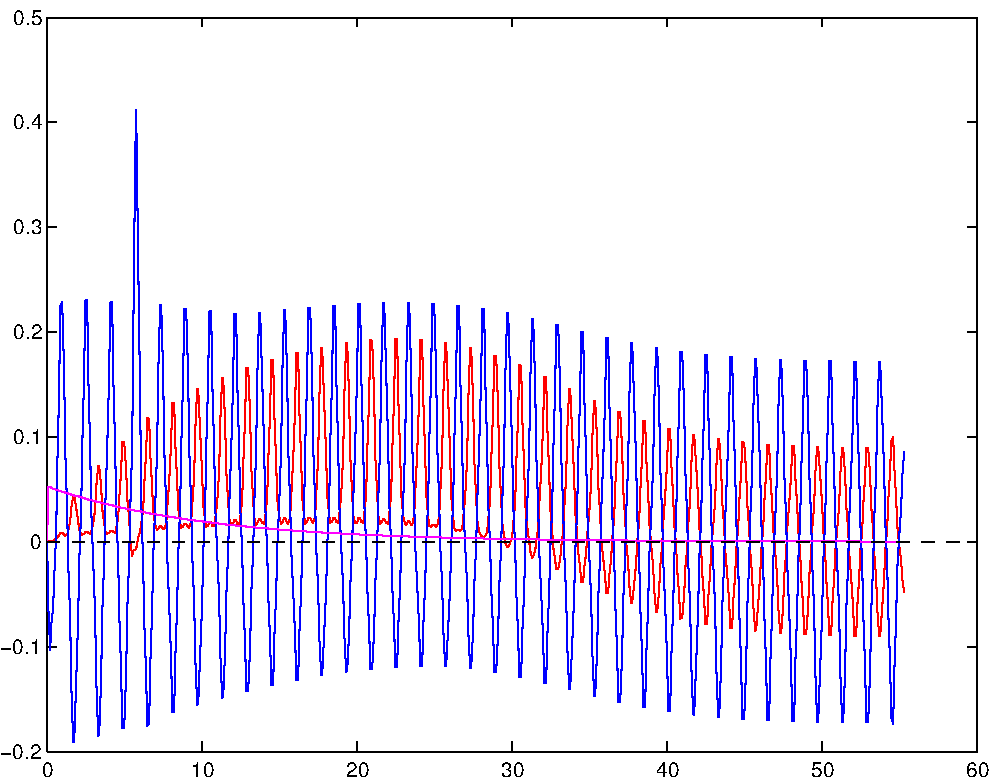
\includegraphics[scale=.27]{figures/velocities4.pdf}
 \label{Fig:Results4b}
 }
 \subfigure[]{
 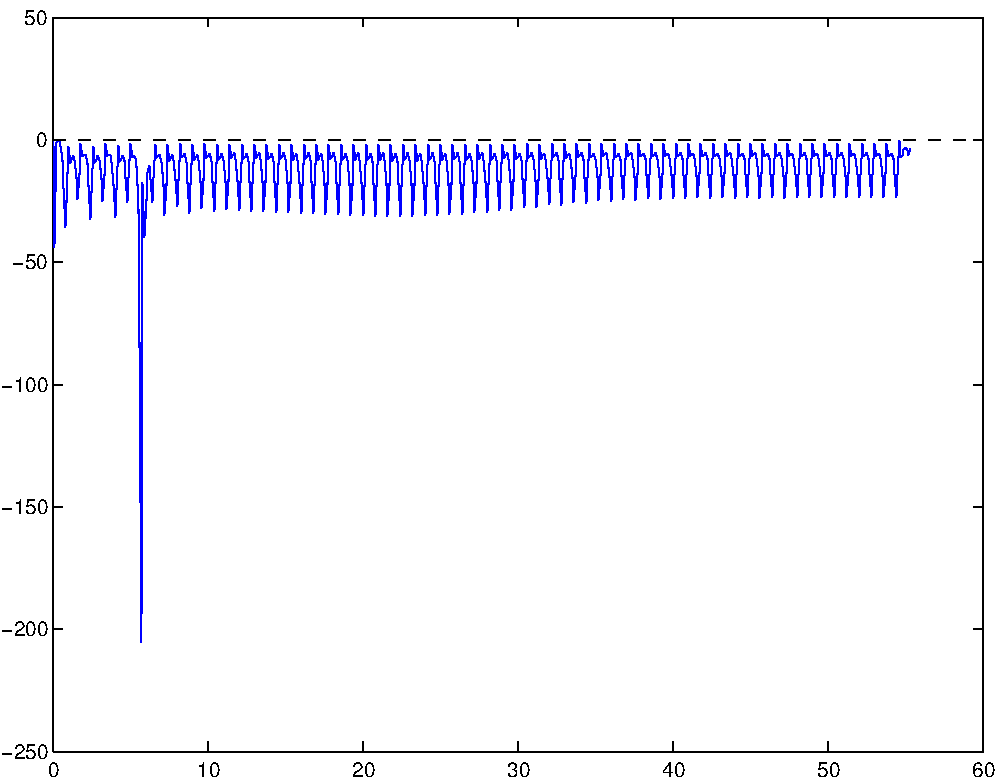
\includegraphics[scale=.27]{figures/objective4.pdf}
 \label{Fig:Results4c}
 }
 \caption[]{\label{Fig:Results4}\small{The behavior of our system in the fourth simulation, with the same graphical conventions as in Fig.~\ref{Fig:Results1}. The robot is following a trajectory similar to the one of Fig.~\ref{Fig:Results3}. After a few footsteps, a strong perturbation is applied to the CoM, inducing a peak in the velocities graph (Fig.~\ref{Fig:Results4b}) and in the cost function value (Fig.~\ref{Fig:Results4c}). The perturbation is quasi-instantly recovered.}}
 \end{figure*}

We have already explained how a local linearization is made to maintain the QP formulation. The performance of this linearization depends of the distance traveled inside the horizon, which depends on the velocity of the robot and the size of the horizon. In Fig.~\ref{Fig:Results5}, we can see the linearized and real features trajectories for a given CoM trajectory. As expected, close to the beginning (the linearization point) the trajectories are quite similar, while the final positions differ much more. This is an extreme situation, since usual metric displacements in the horizon are much smaller than this one. In any case, horizon displacements are bigger when the visual errors are bigger (the robot is far from the desired position) in which case the robot just needs a tendency. But when the errors are getting smaller, the robot needs more precision. In this case, displacements in the horizon becomes smaller so that the difference between the real model and the linearized one becomes negligible.

\begin{figure}[ht]
 \centering
 %\subfigure[]{
 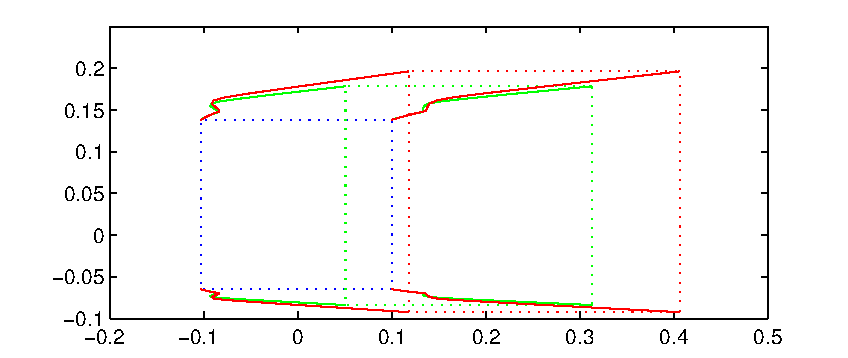
\includegraphics[scale=.6]{figures/comparison_linearization.pdf}
 %\label{Fig:Results2a}
 %}
 % \subfigure[]{
 %\includegraphics[scale=.6]{comparison_linearization_com.pdf}
 %\label{Fig:Results2b}
 %}
 \caption{\label{Fig:Results5}\small{In this figure, we show the trajectory of the visual features in one iteration of the QP, and compare the evolution of the features obtained by the linearization model (green lines) and features obtained by the non-linear model (red lines).}}
 \end{figure}

Due to the walking nature, we have oscillations in the features trajectories. If we use instantaneous errors measurements, the system will never converge, due to these oscillations. One of the main advantages of using MPC is that it naturally filters these oscillations. It is remarkable that, in comparison with~\cite{DuneIROS2010}, we do not need to model explicitly the sway motion of the robot and the resulting motion of the visual features. The system could oscillate inside the horizon (and it does), but at the end, the optimal control is taken without oscillations (Fig.~\ref{Fig:Results6}).

\begin{figure}[ht]
 \centering
 \subfigure[]{
 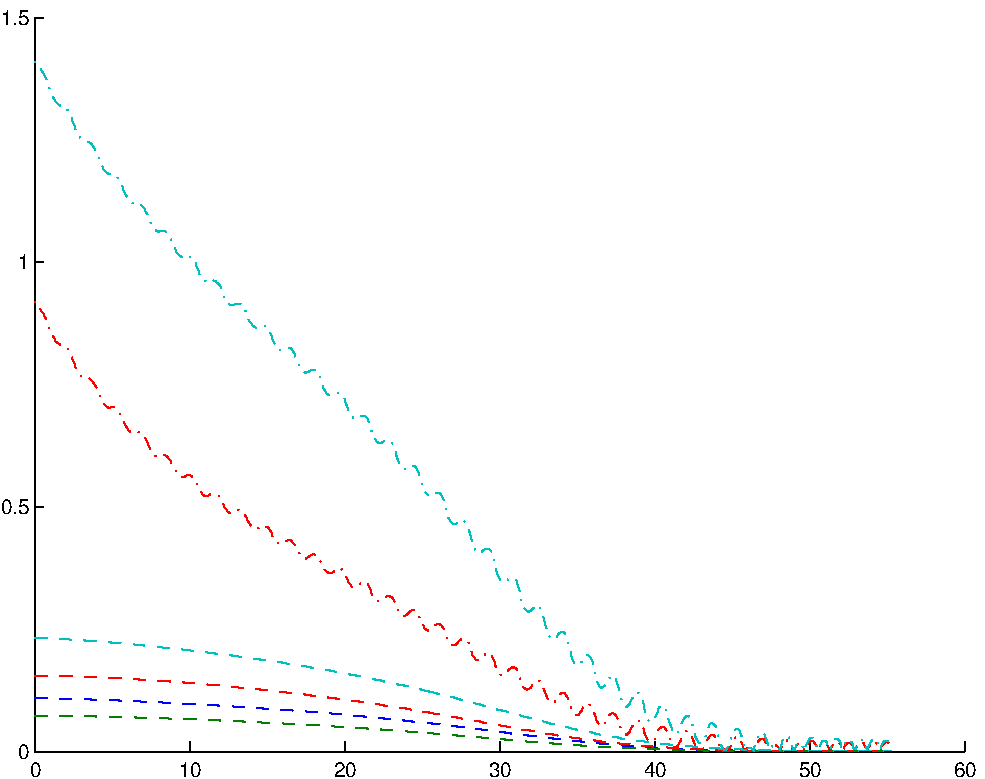
\includegraphics[scale=.23]{figures/instantaneus_errors.pdf}
 \label{Fig:Results6a}
 }
  \subfigure[]{
 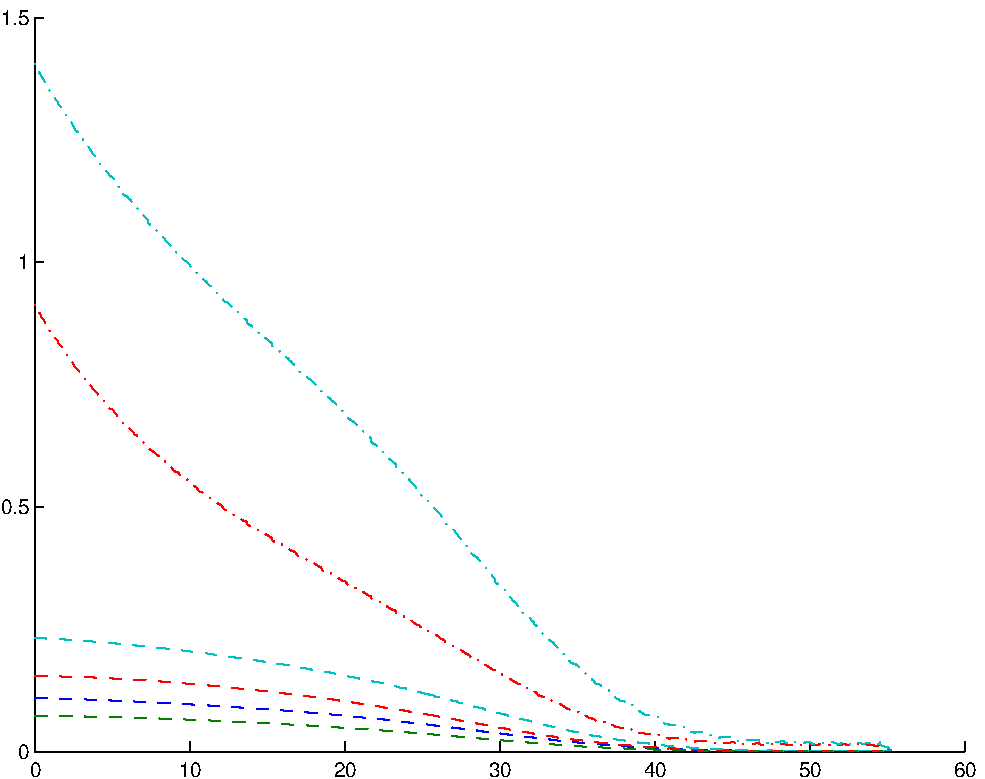
\includegraphics[scale=.23]{figures/horizon_errors.pdf}
 \label{Fig:Results6b}
 }
 \caption[]{\label{Fig:Results6}\small{Evolution of the errors for the $u,v$ components of each feature, in the second simulation. In \ref{Fig:Results6a}, we depict the instantaneous errors along time, and in \ref{Fig:Results6b}, we depict the errors estimated in the horizon (i.e. individual terms of Eq.~ \ref{Eq:MinVisualFeatures2}, normalized by the size of the horizon). Observe that the sway motion of the robot induces oscillations of the $v$ components in the instantaneous errors, and that these oscillations are not present in the errors estimated in the horizon window.}}
 \end{figure}

\section{Conclusion}
\label{sec:conclusions}
Since the original proposal for walking generation proposed in~\cite{Kajita2003}, most of the efforts in the literature have focused in dynamical balance and stability. In this paper, we have proposed a novel approach to close the control loop by introducing visual information into the walking pattern generation. Our online pattern generator integrates the regulation of the relative pose of 3D image features while simultaneous ensuring safety and stability. In order to keep the optimization formulation as a QP, the perspective projection equations have been linearized around the features positions at the beginning of each cycle. However, our current approach uses 3-D information that strongly depends on the localization. As a future work, we wish to drop the need of 3-D information by predicting the image positions of the landmarks in terms on the velocity of the robot in the horizon (IBVS); we also plan to perform real experiments on the HRP-2 humanoid platform.


% Using planning
\chapter{Planning} 
\label{Chap:Visual-Planning}

\section{Global planning with visibility constraints}
%==================================================================

\label{sec:globalplanning}

\begin{figure}[h]
\centering
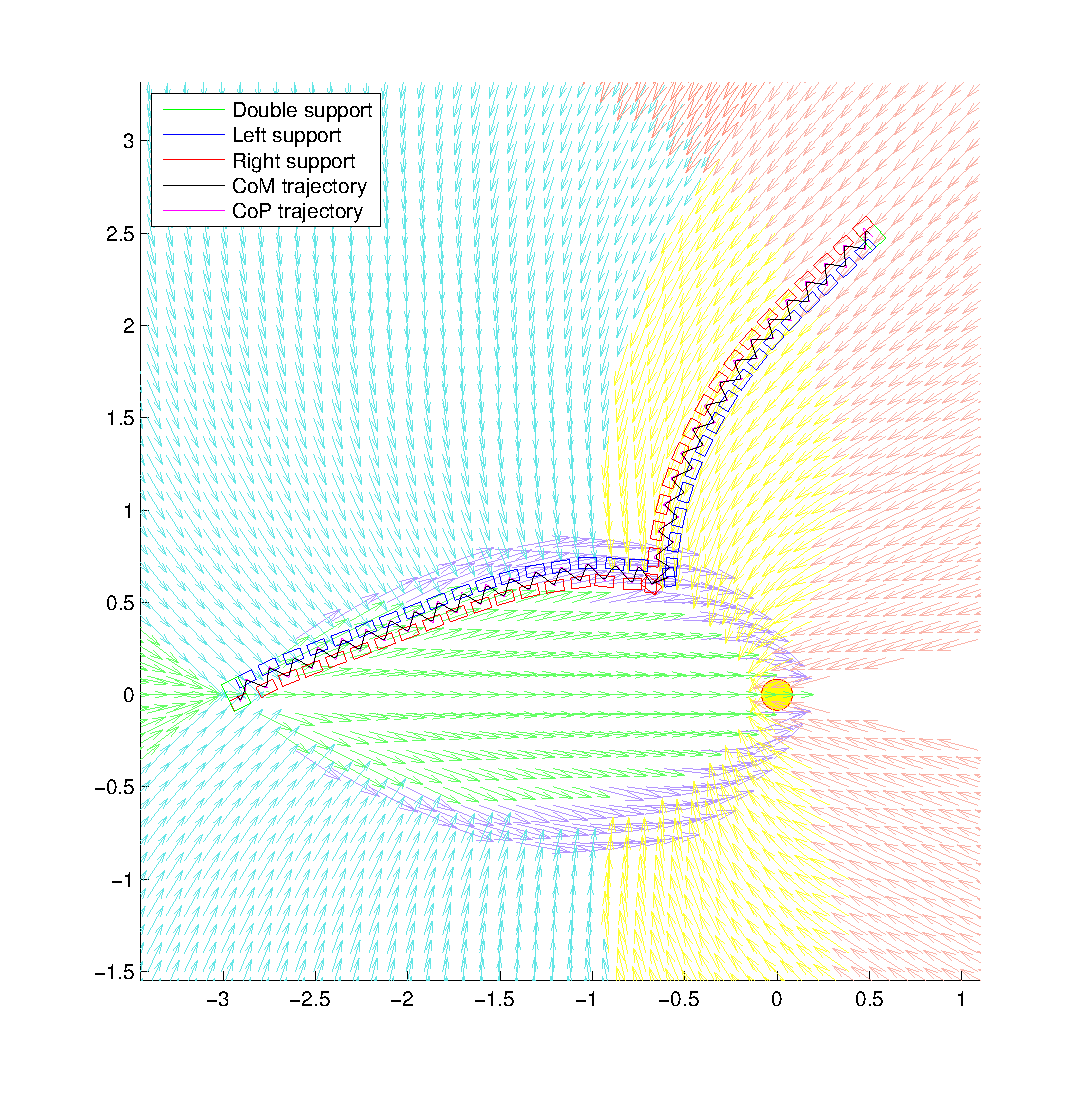
\includegraphics[scale=0.425]{figures/steps6.pdf}
\caption{Vector fields generated by optimal trajectories planned with visibility constraints for a non-holonomic robot~\cite{Salaris:2010}. To each color is associated a family of global paths that reach the goal (at $(-3,0)$) according to the current configuration of the robot while keeping the landmark (yellow disk) visible at all times. The footsteps, CoM and CoP trajectories for the humanoid robot are all depicted as indicated in the upper box.}
\label{fig:steps6}
\end{figure}

For visual servoing, localization, surveillance, or any robotic task based on the observation of visual cues, it is important to ensure that the robot under control does not lose sight of the landmark(s) used as a visual reference. Hence, several works have been proposed to provide motion planners that guarantee landmark visibility, mainly for wheeled robots.

With this concern in mind, we borrow one such global planner, described in~\cite{jib-IJHR2010},  as a base tool for generating paths that guarantee to enforce the required visual constraints while giving locally optimal trajectories in distance. This base planner for humanoid robots uses as an underlying model of motion, a disk-shaped non-holonomic Differential Drive Robot (DDR). In~\cite{jib-IJHR2010}, if a solution path is found for the DDR, it is converted into a solution path for the humanoid robot by generating a footprints sequence coherent with the humanoid dimensions. A nice property inherited from using the DDR model of motion is that the global planner is complete, i.e.  if a solution exists, it will give one, otherwise, it will say so.

However, even if, locally, the used motion primitives are optimal in distance, this approach does not necessarily give globally optimal trajectories. We will not detail the complete methodology here, but we recall the basic results hereafter.

The aforementioned algorithm takes as an input a 2D map of the environment, with its obstacles and visual landmarks, an initial configuration of the robot in the plane, $(x_A,y_A,\theta_A)$, and a final (goal) configuration in the plane, $(x_B,y_B,\theta_B)$. Its output is a set of footprints in the plane to be followed by the robot. The building of this path follows a classical recursive strategy: A roadmap is built over the free space, which includes both, points free of collision with the obstacles in the environment and points that are not within the shadows cast by the landmarks. Then, the initial and final configurations are tested, to check whether the optimal primitives of~\cite{Salaris:2010} can connect them without colliding forbidden regions. If the computed path is without collision, then the algorithm ends, otherwise the holonomic shortest path on the roadmap from the initial configuration to the final (if it exists) is divided in two parts by its middle point, and the whole process is repeated on the two sub-parts. 

The resulting path is made of several parts, each one corresponding to a locally optimal path given from~\cite{Salaris:2010} (made of a combination of straight lines, logarithmic spirals and in-site rotations). This allows to define a set of $S$ sub-segments to be performed by the robot along locally optimal paths, which will be referred to as $(p^s,q^s)$, for $s=1\dots S$~:
$$
p^s = (x_p^s,y_p^s,\theta_p^s)^T \; ; \; q^s = (x_q^s,y_q^s,\theta_q^s)^T,
$$

with $p^s$ the initial configuration and $q^s$ the final one. The complete computed path is executed by reaching the successive sub-goals $q^s$.


%==================================================================
\section{Defining a local reference trajectory}
%==================================================================

\label{sec:reftrajectories}

Let us focus on the execution of each sub-path $s$. Suppose that we start with the robot at some configuration close to $p^s$ (see Fig.~\ref{fig:paths}), because localization may not be perfect, and suppose that we want to reach the final configuration or sub-goal $q^s$, as determined in~\cite{jib-IJHR2010}.

\subsection{Adapting the reference trajectory for the MPC}

Without loss of generality, we suppose that the object of interest to be kept at sight by the robot is located at $\mathbf L^s = (0,0)$. In all the following, $x,y,\theta$ will refer to coordinates w.r.t a global frame centered at this origin.

It is noteworthy that, given the sub-goal $q^s =(x_q^s,y_q^s,\theta_q^s)^T$ to reach, and the landmark it is associated to, the work of~\cite{Salaris:2010} gives us a full synthesis of optimal paths in free space. This synthesis can be represented as a mapping $\sigma$:
$$
\begin{array}{cccccc}
\sigma & : & \mathbb{R}^2 & \mapsto & \mathbb{S}^1 \times \mathbb{R}^2\\
& & (x,y) & \rightarrow & (\theta^*(x,y),v^*(x,y),\omega^*(x,y))
\end{array}
$$

where $\theta^*(x,y)$ is the orientation the robot (viewed as a nonholonomic cart)  should have in order to start walking along the shortest path to $q^s$, from its current position $(x,y)$. The pair $(v^*(x,y),\omega^*(x,y))$ are the instantaneous (reference) velocities needed to be applied to follow the shortest paths. Without loss of generality, we can suppose that $v^*(x,y)=0$ (for in-site rotations) or $v^*(x,y)=\pm 1$ (elsewhere). Given the linear velocity $v^*(x,y)$, $\omega^*(x,y)$ is defined in function of the nature  of the path segment,
$$
\left\{
\begin{array}{cccc}
 \omega^*(x,y) & = & 0 & \mbox{(straight line)}\\
  & = & \pm\frac{\sin(\phi_{max})}{\sqrt{x^2+y^2}} & \mbox{(spiral)},\\
\end{array}
\right.
$$

where $\phi_{max}$ is the maximal bearing angle possible for the landmark, given the sensor and robot characteristics.

Our claim is that the knowledge of optimal policies at each point allows some flexibility when generating a walking pattern, by optimizing the footprint positions and  the CoM trajectory ``around'' the nominal path output from the planner, by using these policies within the pattern generation.

\begin{figure}
\input{figures/config.pdf_t}
\caption{From a configuration $(x,y,\theta)$ and its corresponding position $(x,y)$, and a sub-goal $q^s= (x_q^s,y_q^s,\theta_q^s)$ to reach, the optimal path (dashed line) is the one we want the humanoid robot to follow. For that, we use the tangent orientation $\theta^*(x,y)$ to this path. Because of the errors in control or localization, this optimal path may be different from the shortest path (solid line) computed from the first configuration $p^s= (x_p^s,y_p^s,\theta_p^s)$.
%For the linearization purposes, and given that $(x,y)$ will be variable, we will use a nominal shortest path (solid line) from a close, fixed configuration $p^s= (x_p^s,y_p^s,\theta_p^s)$.
\label{fig:paths}}
\end{figure}

In pattern generation algorithms such as~\cite{HerdtAR2010}, the cost function within the Model Predictive Control (MPC) window uses the configurations of the CoM. Here, focusing more specifically on the $(x,y,\theta)$ CoM coordinates, we handle as an input of the algorithm a reference trajectory to be followed, and a synthesis of shortest paths leading to a given objective, as a direct output from~\cite{Salaris:2010}. As depicted in Fig.~\ref{fig:paths}, at each configuration evaluated within the MPC, two forces should apply through the optimization scheme: one driving the robot to the ``correct'' orientation $\theta^*(x,y)$, and one making the velocities follow the shortest path, $(v(x,y),\omega(x,y))$. Also, a strong visibility constraint should apply, to ensure the object of interest to stay visible. In Fig.~\ref{fig:fieldNoLateral}, we give an illustration of the shortest paths synthesis from~\cite{Salaris:2010}, displayed through the local orientations of optimal paths at each point of the plane, given the objective to reach (``end point'') and the landmark to keep in sight. 


%==================================================================
%\subsection{Tracking a single reference trajectory}
%==================================================================

%\label{subsection-singleref}

%In that case, we would track the reference path from $p^s$ to $q^s$; this has the advantage of being rather simple to express, I believe. Consider the reference path from $p^s$ to $q^s$; generate a corresponding sampled trajectory  $x_{ref}(k\tau),y_{ref}(k\tau),\theta_{ref}(k\tau)$, then stack them into vectors $C^x_{ref},C^y_{ref},C^\theta_{ref}$. Note that from the same analysis, we could also reinforce the tracking of the desired trajectories by including reference velocities, 

%$$
%\left\{
%\begin{array}{ccc}
%\dot{x}_{ref}(k\tau) & = & v \cos(\theta_{ref}(k\tau)) \\
%\dot{y}_{ref}(k\tau) & = & v \sin(\theta_{ref}(k\tau)) \\
%\dot{\theta}_{ref}(k\tau) & = & \omega(v,x_{ref}(k\tau),y_{ref}(k\tau)) \\
%\end{array}
%\right.
%$$

%where $v$ is a reference linear velocity, and $\omega(v,x_{ref}(k\tau),y_{ref}(k\tau))$ directly deduced from the synthesis. Similarly to positions, these references velocities could be stacked into $\dot{C}^x_{ref},\dot{C}^y_{ref},\dot{C}^\theta_{ref}$.

%We would introduce directly this desired trajectory in the pattern generator, while keeping the decoupled formulation of~\cite{HerdtIROS2010}, for the $x,y$ position on the one hand, and for the $\theta$ angle, on the other. Hence,

%{\small
%\begin{eqnarray}
%\nonumber
% \min && \dfrac{\alpha}{2} \left\| C^x_{i+1} - C^x_{ref} \right\|^2 + \dfrac{\alpha}{2} \left\| C^y_{i+1} - C^y_{ref} \right\|^2 \\
%\nonumber
%&& + \dfrac{\beta}{2} \left\| \dot{C}^x_{i+1} - \dot{C}^x_{ref} \right\|^2 + \dfrac{\beta}{2} \left\| \dot{C}^y_{i+1} - \dot{C}^y_{ref} \right\|^2 \\
%\nonumber
%&& + \dfrac{\gamma}{2} \left\| F^x_{i+1} - Z^x_{i+1} \right\|^2 + \dfrac{\gamma}{2} \left\| F^y_{i+1} - Z^y_{i+1} \right\|^2 \\
%&& + \dfrac{\epsilon}{2} \left\| \dddot{C}^x_{i} \right\|^2 + \dfrac{\epsilon}{2} \left\| \dddot{C}^y_{i} \right\|^2,
%\end{eqnarray}
%}

%and for the angular position,

%{\small
%\begin{eqnarray}
%\nonumber
% \min && \dfrac{\alpha}{2} \left\| C^{\theta}_{i+1} - C^{\theta}_{ref} \right\|^2 + \dfrac{\beta}{2} \left\| \dot{C}^{\theta}_{i+1} - \dot{C}^{\theta}_{ref} \right\|^2 \\
%&& \dfrac{\gamma}{2} \left\| \sum (f^{\theta}_i - c^{\theta}_i) \right\|^2 
%\label{eq-opt-orientations}
%\end{eqnarray}
%}

%where $C^{\alpha}_{ref}$ with $\alpha \in \{x,y,\theta\}$ is the reference trajectory in the horizon, extracted from the trajectory generated with the planner \cite{HayetIJHR2010}.

%Note that the same process can be applied by considering, instead of $p^s$, the point corresponding to the current robot position. This would be a first, cheap way to adapt the reference trajectory. In both cases, the orientations would have been computed beforehand by Eq.~\ref{eq-opt-orientations}.

\begin{figure*}[ht]
\vspace{2 mm}
\hspace{5 mm}
 \subfigure[Motion direction field resulting from the synthesis of~\cite{Salaris:2010}.]{
  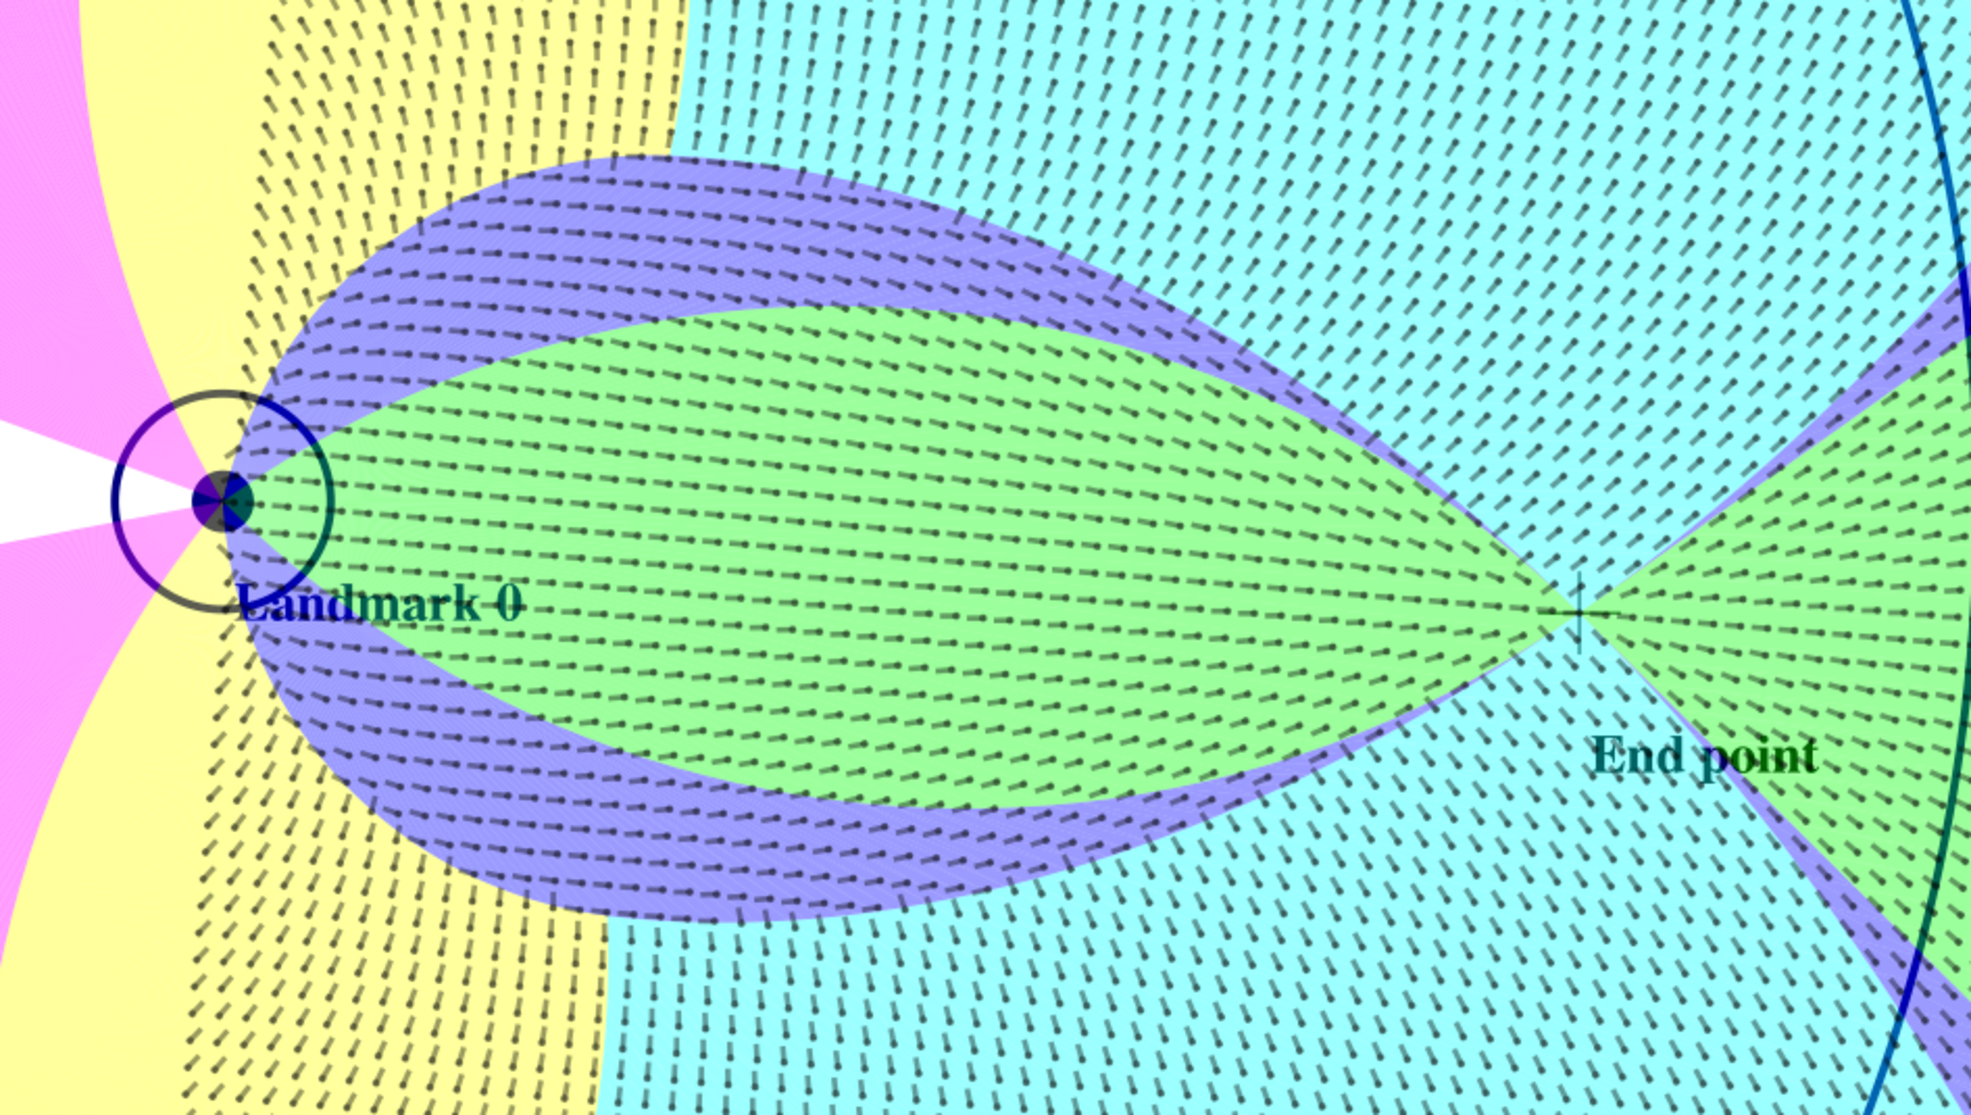
\includegraphics[scale=0.213]{figures/noLateral}
   \label{fig:fieldNoLateral}
   }
   \hspace{15 mm}
 \subfigure[Motion direction field with lateral motions.]{
  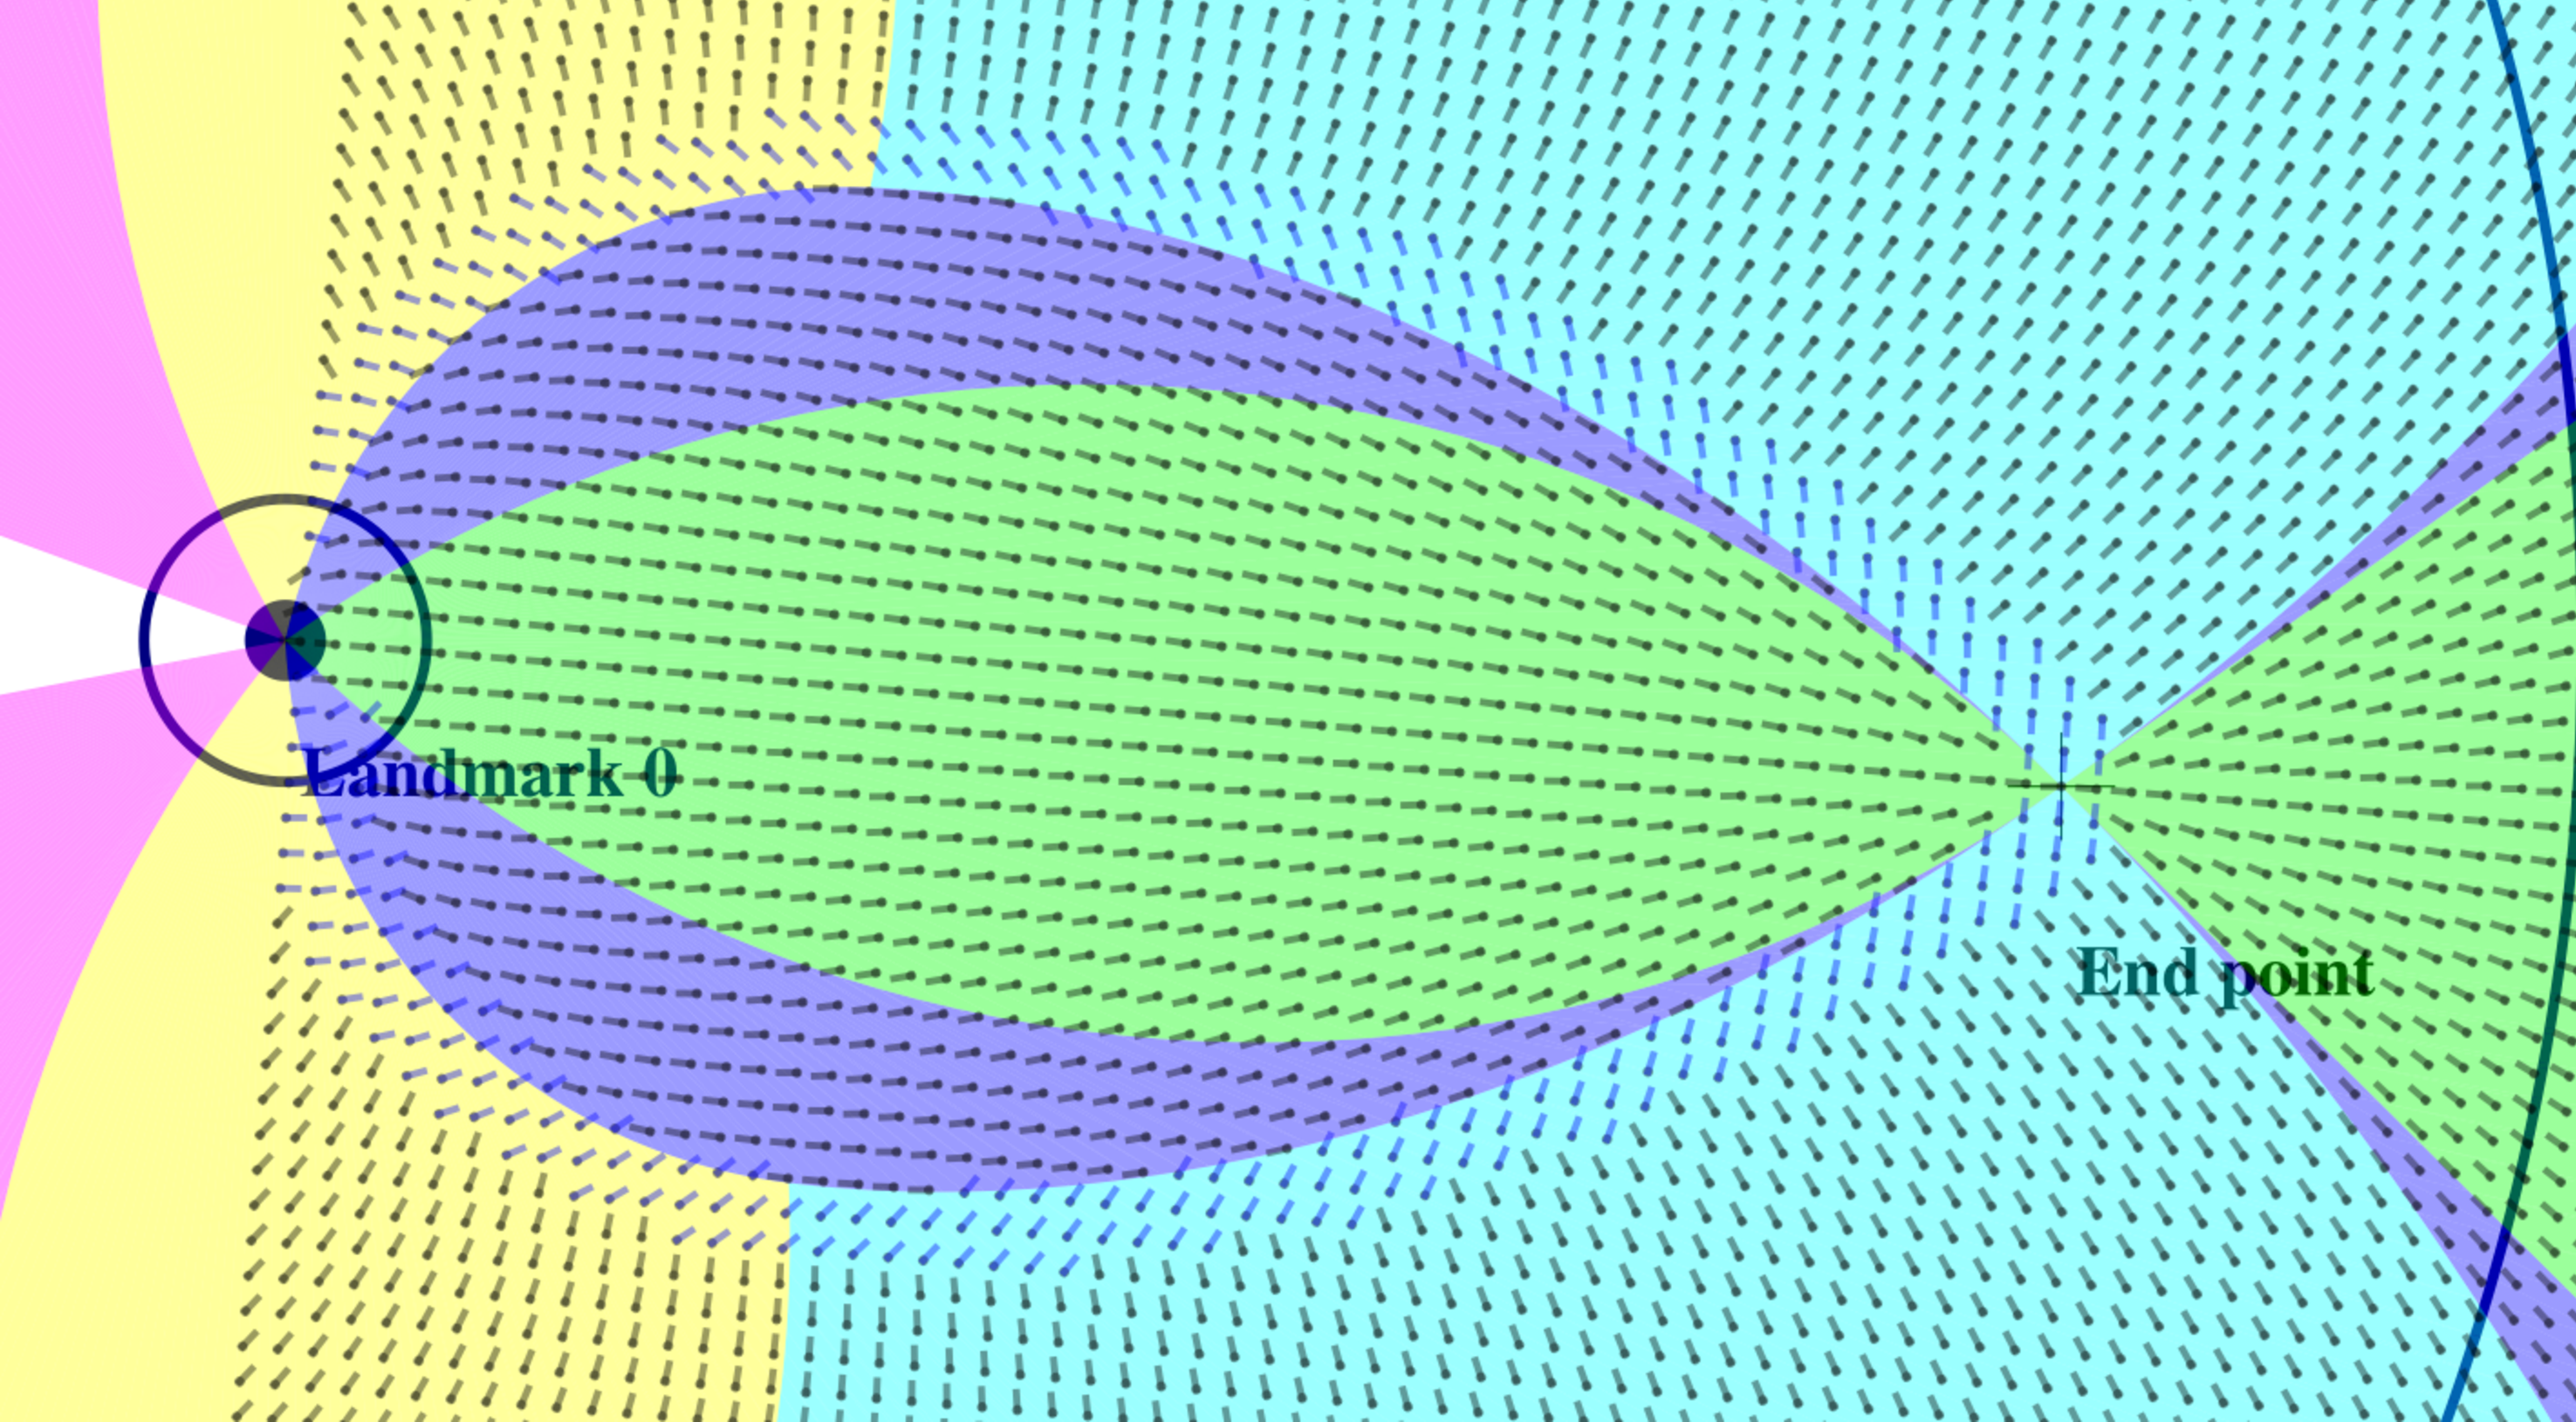
\includegraphics[scale=0.145]{figures/useLateral}
   \label{fig:fieldUseLateral}
   }
 \caption[]{Visualization of optimal motion directions $\theta^*(x,y)$. Both figures indicate the nature of optimal paths with the filling colors, and the tangent direction to the optimal curve all over a grid defined around the final point. In Fig.~\subref{fig:fieldNoLateral}, the field is computed directly from the primitives of~\cite{Salaris:2010}. The locus of in-site rotations is identifiable at the dark blue zone border. In Fig.~\subref{fig:fieldUseLateral}, the non-holonomy behavior close to this locus is replaced by lateral motions.\label{fig:field}}
\end{figure*}

\subsection{Quadratic programming MPC}

\label{sec:wpg}

Since the work of~\cite{Kajita2003}, walking pattern generation algorithms have focused on determining constant-height (at height $h$) trajectories of the CoM with piecewise-constant jerks time profiles. These profiles are computed by a MPC scheme for time intervals of length $T$, under a simplified cart-plane mechanical model simulated for a near time horizon,  within $N$ time intervals. In this paper, we follow a similar approach and will refer to the time interval indices as $k$. 

To produce balanced and stable movements,~\cite{Kajita2003} formulates the dynamics of the CoM, axis per axis, as   

\begin{equation}
\left\{
\begin{array}{ccc}
 \hat{x}_{k+1} &=& A \hat{x}_k + J \dddot{x}_k\\
 \xi^x_{k} &=& Z \hat{x}_k 
\end{array}
\right.
\label{Eq:dynamic}
\end{equation}

for the example of the $x$ axis, where vectors $\hat{x}_{k} = \left( x_k, \dot{x}_k, \ddot{x}_k \right)^{\transpose}$ stack the position, velocity and acceleration of the CoM along the $x$-axis and ${\xi}^x_k$ is the CoP $x-$coordinate, both at time $k$. The matrices $A$, $J$, $Z$ are defined as

\begin{equation*}
A = \left(
\begin{matrix}
1 & T & \frac{1}{2}T^2 \\
0 & 1 & T \\
0 & 0 & 1
\end{matrix}
\right) \text{, }
J = \left(
\begin{matrix}
\frac{1}{6}T^3 \\
\frac{1}{2}T^2 \\
T
\end{matrix}
\right) \text{ and }
Z = \left(
\begin{matrix}
1 \; 0 \; \frac{h}{g} \\
\end{matrix}
\right),
\end{equation*}

where $g$ is the gravity. To predict the CoM trajectories within the next $N$ time intervals, the dynamics is applied recursively, starting from the initial position $\hat{x}_k$, in function of the sequence of jerk values to be applied, $\dddot{C}^{x} = (\dddot{x}_k, \dddot{x}_{k+1},...,\dddot{x}_{k+N-1})^{\transpose}$, where $P_{ps}$ and $P_{pu}$ are constant matrices,

\begin{equation}
 \label{Eq:PosCMHorizon}
 C^x_{k+1} \stackrel{\mbox{\tiny def}}{=} \left(
 \begin{matrix}
  x_{k+1} &
  \hdots &
  x_{k+N}
 \end{matrix}
 \right)^{\transpose} = P_{ps} \hat{x}_k + P_{pu} \dddot{C}^{x} _k.
\end{equation}

Similar expressions can be obtained for the $y$ component and for the velocity and acceleration of the CoM.

As an evolution of the original work of Kajita~\cite{Kajita2003}, where the footsteps positions (and, correspondingly, the CoP positions) are fed to the pattern generation, the work of~\cite{HerdtAR2010} introduced automatic footstep planning, and reduced the necessary input to a simple stack of reference velocities $(\dot{X}_{k+1}^{ref},\dot{Y}_{k+1}^{ref})$. This leads to the optimization problem:

{\scriptsize
\begin{eqnarray}
\nonumber
 \underset{U_{k}}{\min} \; && \dfrac{\alpha}{2} \left\| \dddot{C}_k^{x} \right\|^2 + \dfrac{\beta}{2} \left\| \dot{C}_{k+1}^{x} - \dot{X}_{k+1}^{ref} \right\|^2
 + \dfrac{\gamma}{2} \left\| Z_{k+1}^x - Z_{k+1}^{x_{ref}} \right\|^2 \\
 && + \dfrac{\alpha}{2} \left\| \dddot{C}_k^{y} \right\|^2 + \dfrac{\beta}{2} \left\| \dot{C}_{k+1}^{y} - \dot{Y}_{k+1}^{ref} \right\|^2
 + \dfrac{\gamma}{2} \left\| Z_{k+1}^y - Z_{k+1}^{y_{ref}} \right\|^2
\label{Eq:MinJerk}
\end{eqnarray}
}
with the variables to optimize kept in the vector $U_{k} \stackrel{\mbox{\tiny def}}{=}  \left( (\dddot{C}_k^{x})^ \transpose, (X_{k}^{f})^ \transpose, (\dddot{C}_k^{y})^ \transpose, (Y_{k}^{f})^ \transpose \right)^{\transpose}$. The ZMP references $Z_{k+1}^{x_{ref}},Z_{k+1}^{y_{ref}}$ depend linearly on the variables $X_{k}^{f},Y_{k}^{f}$ which are the position of the next footsteps in the horizon.

As the sequence of CoP positions $Z_{k+1}^x = [ {\xi}^x_{k+1} \; \cdots \; {\xi}^x_{k+N}]$ is linear in the variables to optimize (from Eq.~\ref{Eq:dynamic}), the problem is a Quadratic Program (QP) 

\begin{equation}
 \underset{U_k}{\min} \; \dfrac{1}{2} U_k^{\transpose} Q_k U_k + p_k^{\transpose} U_k,
\label{Eq:QP}
\end{equation}

under linear constraints arising, among others, from the inclusion of the CoP inside the support polygon~\cite{HerdtAR2010}.

\subsection{Using the optimal path synthesis within the MPC}

Instead of utilizing in the Equation~\ref{Eq:MinJerk}, a single, constant reference trajectory, defined by the plan computed from $p^s$ to $q^s$, and from which $(\dot{X}_{k+1}^{ref},\dot{Y}_{k+1}^{ref})$ would be evaluated, our idea is to use explicitly the mapping $\sigma$ described above. This way, we can adapt the path execution and find the shortest path to the next sub-goal from any point, not just from $p^s$. As explained above, one can  associate to any $x,y$ the tangent $\theta^*(x,y)$ to the shortest path. One way to enforce the tracking of these shortest paths is to set as a reference velocity (supposing we are following a piece of curve with $v=1$) defined in the time horizon ($l>k$, where $k$ is the current time index):
$$
\begin{array}{ccc}
\dot{x}^{ref}_l =  \cos(\theta^*(x_l,y_l)) & \; & \dot{y}^{ref}_l =  \sin(\theta^*(x_l,y_l)) \\
\end{array}
$$

that depends (non-linearly) on $x_l,y_l$. The idea is to use these -- variable -- reference velocities inside the terms of the pattern generator QP. However, as this mapping is non-linear, a direct use would make us lose the QP form, that allows an efficient resolution of the problem. Because the mapping $\theta^*(x,y)$ has not always an analytic form we evaluate it numerically on a fine scale grid inside the zone of operation of the robot, as pre-computed values, and we also estimate numerically the partial derivatives $\frac{\partial \theta^*(x,y)}{\partial x},  \frac{\partial \theta^*(x,y)}{\partial y}$.

This way, we can approximate each of these reference velocities, at time position $l$ within the optimization time window, by performing a linearization of $\theta^*$  around a reference position $(x^0,y^0)$, i.e.,
$$
\begin{array}{ccc}
\theta^*(x_l,y_l) & \approx & \theta^*(x^0_l,y^0_l)  \\
& & + \frac{\partial \theta^*(x^0,y^0)}{\partial x} (x_l-x^0) + \frac{\partial \theta^*(x^0,y^0)}{\partial y} (y_l-y^0).
\end{array}
$$

Note that the linearization point $(x^0,y^0)$ is chosen in the aforementioned grid of pre-computed values $(\theta^*(x,y),\frac{\partial \theta^*(x,y)}{\partial x},  \frac{\partial \theta^*(x,y)}{\partial y})$, at the closest point to the first (current) CoM position. This grid is depicted in the background of Figs.~\ref{fig:steps6}, \ref{fig:field}, \ref{fig:steps10} among others. To simplify the notation, let us write
$$
\theta^0 \stackrel{\mbox{\tiny def}}{=}  \theta^*(x^0,y^0),\;
\frac{\partial \theta^0}{\partial x} \stackrel{\mbox{\tiny def}}{=} \frac{\partial \theta^*(x^0,y^0)}{\partial x},\;
\frac{\partial \theta^0}{\partial y} \stackrel{\mbox{\tiny def}}{=}  \frac{\partial \theta^*(x^0,y^0)}{\partial y}. 
$$


Then, we re-write the errors to the reference velocities at each time step $l>k$, as a linear function of $\dot{x}_l,\dot{y}_l,x_l,y_l$
$$
\left\{
\begin{array}{ccc}
\dot{x}_l-\dot{x}^{ref}_l & = & \dot{x}_l - v\cos(\theta^0)\\
&& + v\sin(\theta^0) \frac{\partial \theta^0}{\partial x}  (x_l-x^0)\\
&& + v\sin(\theta^0) \frac{\partial \theta^0}{\partial y}  (y_l-y^0),\\
\dot{y}_l-\dot{y}^{ref}_l & = & \dot{y}_l - v\sin(\theta^0_l)\\
&& - v\cos(\theta^0) \frac{\partial \theta^0}{\partial x}  (x_l-x^0)\\
&& - v\cos(\theta^0) \frac{\partial \theta^0}{\partial y}  (y_l-y^0),
\end{array}
\right.
$$ 

and by stacking the errors within the horizon window as in Eq.~\ref{Eq:PosCMHorizon}, we get the following 
linear relations

{\small
\begin{eqnarray}
\nonumber
 \dot{C}_{k+1}^{x}  - \dot{X}_{k+1}^{ref} & = &    \dot{C}_{k+1}^{x} -   \dot{C}_{k+1}^{0,x}  + A^x_{0} C_{k+1}^{x}  + B^x_{0} C_{k+1}^{y},\\
 \dot{C}_{k+1}^{y} - \dot{Y}_{k+1}^{ref} & = &   \ \dot{C}_{k+1}^{y} - \dot{C}_{k+1}^{0,y} + A^y_{0} C_{k+1}^{x} + B^y_{0}  C_{k+1}^{y},
 \label{eq-velref-linear}
 \end{eqnarray}}

where $A^x_{0},B^x_{0},A^y_{0},B^y_{0}$ are diagonal matrices collecting the terms $v\sin(\theta^0_l) \frac{\partial \theta^0_l}{\partial x}$ and alike. Then, the walking pattern generation is formulated exactly as in Eq.~\ref{Eq:MinJerk}, with the reference velocities given by Eq.~\ref{eq-velref-linear}, and with the optimization variable being $U_{k}$,
%$U_{k} \stackrel{\mbox{\tiny def}}{=}  \left( (\dddot{C}_k^{x})^ \transpose, (X_{k}^{f})^ \transpose, (\dddot{C}_k^{y})^ \transpose, (Y_{k}^{f})^ \transpose \right)^{\transpose}$ 
leading to a canonical Quadratic Program (QP) similar to Eq.~\ref{Eq:QP}.

%{\scriptsize
%\begin{eqnarray}
%\nonumber
% \min\limits_{\dddot{C}^x_k,Z^x_{k+1},\dddot{C}^y_k,Z^y_{k+1}}  &&  \dfrac{\beta}{2} \left\| \dot{C}_{k+1}^{x}  - \dot{X}_{k+1}^{ref} \right\|^2 + \dfrac{\beta}{2} \left\| \dot{C}_{k+1}^{y}  - \dot{Y}_{k+1}^{ref} \right\|^2 \\
%\nonumber
%&& + \dfrac{\gamma}{2} \left\| Z^{x_{ref}}_{k+1} - Z^x_{k+1} \right\|^2 + \dfrac{\gamma}{2} \left\| Z^{y_{ref}}_{k+1} - Z^y_{k+1} \right\|^2 \\
%&& + \dfrac{\alpha}{2} \left\| \dddot{C}_{k}^{x}  \right\|^2 + \dfrac{\alpha}{2} \left\| \dddot{C}_{k}^{y} \right\|^2,
%\label{eq-main-qp}
%\end{eqnarray}
%}

% that can be expressed in terms of $U_{k} \stackrel{\mbox{\tiny def}}{=} \left( (\dddot{C}_k^{x})^ \transpose, (Z_{k+1}^{x_{ref}})^ \transpose, (\dddot{C}_k^{y})^ \transpose, (Z_{k+1}^{y_{ref}})^ \transpose \right)^{\transpose}$ by using Eq.~\ref{eq-velref-linear}, into a canonical Quadratic Program (QP) similar to Eq.~\ref{Eq:QP}.

The constraints arising from the CoP position to be included in the support polygon being non-linear in the feet orientation, we simply set the robot and feet orientations as follows and include the computed values into the QP.

\subsection{Control of the rotation angle}
In order for the robot to be oriented with the tangent to the optimal path, $\theta^0$, and to keep the QP form, we use a decoupled approach for the control of the rotation angles of the CoM and the feet~\cite{HerdtIros2010}. Hence, in a first stage, we optimize the orientations in the MPC time window by  

{\small
\begin{eqnarray}
\nonumber
 \min\limits_{\dddot{C}_k^{\theta},\dddot{F}_k^{\theta}}  &&  \dfrac{\beta}{2} \left\| C_{k+1}^{\theta} - \theta^{0} \right\|^2 + \dfrac{\gamma}{2} \left\| F_{k+1}^{\theta} - \theta^{0} \right\|^2 \\
\nonumber && + \dfrac{\alpha}{2} \left\| \dddot{C}_{k}^{\theta} \right\|^2 + \dfrac{\alpha}{2} \left\| \dddot{F}_{k}^{\theta} \right\|^2,
\end{eqnarray}
}

and then in a second stage, we introduce these angles as constant in the main QP (Eq.~\ref{Eq:MinJerk}). This approach gives us the advantage of introducing constraints like maximum rotation between both feet, between feet and trunk and also a rotation limit to keep the visibility of the landmarks.

%\subsection{Refinement of the angular position}

%\textcolor{blue}{JB:} Will we do something about that?: the idea would be to do a second pass where the $\theta^0$ would be re-evaluated.

%\textcolor{blue}{MG:} You meant the linearization points right, is it still necesary after the clarification?

%=============================================================================================================================================================

\section{Including holonomic behavior}
\label{sec:includingholonomic}

Handling holonomic and non-holonomic behaviors together during locomotion has been previously been discussed in \cite{MombaurHumanoids2008} in a context of motion planning.

One of the most visible disadvantages of the optimal non-holonomic paths given from~\cite{jib-IJHR2010} is the presence of in-site rotations, that are not efficient in terms of footsteps number.
One solution is to use a different formulation of the cost function using weights according to the robot direction and control the head.
But including this vision based control in Eq.~\ref{Eq:MinJerk} is incompatible with a QP formulation.
A strategy we propose here is to take advantage of the fact that the set of points where in-site rotations occur is very well defined geometrically in the plane, as a direct consequence of the synthesis from~\cite{Salaris:2010}. As illustrated in Fig.~\ref{fig:fieldNoLateral}, it is the outer boundary of the partition zone where the shortest paths have to be done as line segments followed by spirals, i.e. the dark blue region of the figure. This curve is made of two parts~\cite{Salaris:2010}, one arc of circle and one piece of logarithmic spiral. Hence, we propose to perform the following: for all points inside the partition regions in contact with this locus, we evaluate its distance in terms of the primitive to be done to reach this locus and modify the reference velocities as follows. 

If the robot is far from the locus of in-site rotations, then the path to follow is continuously derivable and goes either forwards or backwards; in that case, we use the ``non-holonomic behavior'' as described in Section~\ref{sec:reftrajectories}, with the robot orientation controlled to stay close to $\theta^*(x_l,y_l)$,
$$
\begin{array}{c}
\dot{x}^{ref}_l  =  \cos(\theta^*(x_l,y_l)) \;,\; \dot{y}^{ref}_l  =  \sin(\theta^*(x_l,y_l)), \\
\end{array}
$$

and if the robot configuration is close to this locus, then we use instead lateral motions, with orientation $\phi(x_l,y_l)+\pi$, where $\phi(x_l,y_l)=\arctan\frac{y_l}{x_l}$ is the polar angle of $(x_l,y_l)$,
$$
\begin{array}{c}
\dot{x}^{ref}_l  =  -\varepsilon\sin(\phi(x_l,y_l)) \;,\; \dot{y}^{ref}_l  =  \varepsilon\cos(\phi(x_l,y_l)),  \\
\end{array}
$$

where $\varepsilon =\pm1$ in function of the relative position of the goal to reach with respect to the evaluated point. 

In Fig.~\ref{fig:fieldUseLateral}, we illustrate this modification by drawing the lateral motion field with blue arrows, together with the ``non holonomic'' field ``far'' from the locus of in-site rotations. 

%=============================================================================================================================================================
\section{Results}
\label{sec:results}

%=============================================================================================================================================================

In this section, we present three experiments. In the first one, we test the performance of our approach in the absence of localization uncertainty, and with only non-holonomic motion. In the second one, we introduce localization uncertainty. In the last one, we present an improvement to the border behavior with the possibility of holonomic motion. The three experiments have the same set-up, with initial position in $(0.5,2.5)$, landmark position in $(0,0)$ and final position in $(-3,0)$. We chose this trajectory because it makes the robot pass through several regions of the partition and illustrates the border behavior which is one of the problems we found.

In Fig.~\ref{fig:steps6}, we depict the performance in perfect and noiseless conditions. We see that using the planner vector field for driving the robot to the goal produces smooth and stable trajectories of the CoM. However, in real conditions, the robot will not perform the control exactly e.g., because of sliding with the floor. Moreover the robot needs a localization system which will be inherently noisy. To model this situation we perturbed the current position of the CoM with white gaussian noise $\sim \mathcal{N}(0,\sigma^2)$ in each coordinate with $\sigma = 0.2$ and with $\sigma = 10$ degrees for the orientation.

In Fig. \ref{fig:steps10}, we show the behavior in that situation. We can still appreciate a smooth trajectory in the regions far from the border of the dark blue region of the partition, where the vector field is smooth. We also notice the good behavior of the orientation angle mainly because the QP formulation controls it. The main problem of this approach also appears: The discontinuities in the partition regions in which an in-site rotation occurs. Hence, the robot may perform unnecessary maneuvers, involving in-site rotations, which is far from optimal in the case of human walking (Fig.~\ref{fig:steps10zoom}). Moreover, in-site rotations cause high rotation speeds of the feet (Fig.~\ref{fig:velocities10}), which is not desirable from a balance point of view.

\begin{figure}[ht]
\centering
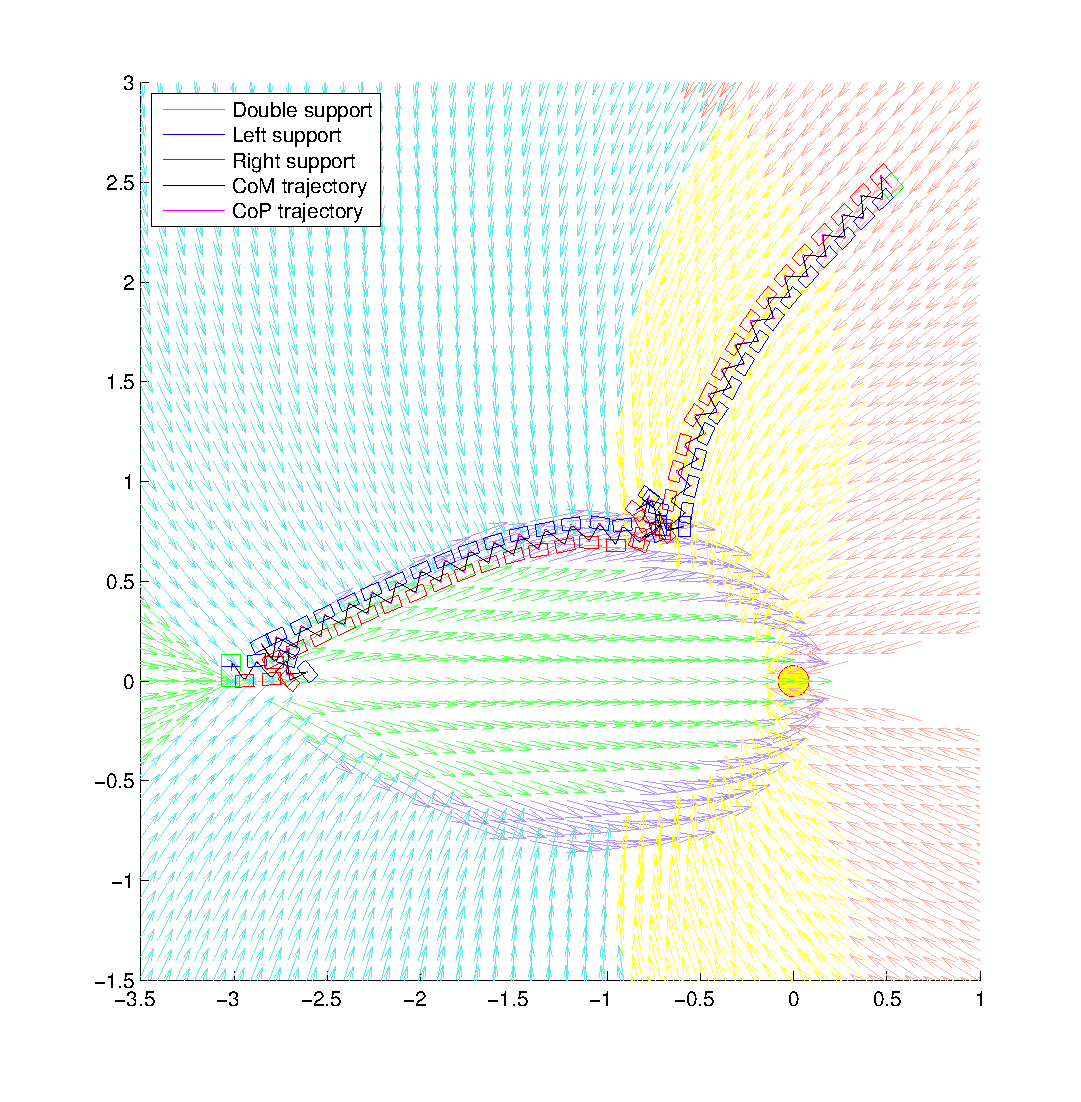
\includegraphics[scale=0.425]{figures/steps10.pdf}
\caption{If the control is not followed well and if we use an imperfect localization system, problems may arise in the borders of the partition, in case of relying on purely non-holonomic behaviors.}
\label{fig:steps10}
\end{figure}

\begin{figure}[ht]
\centering
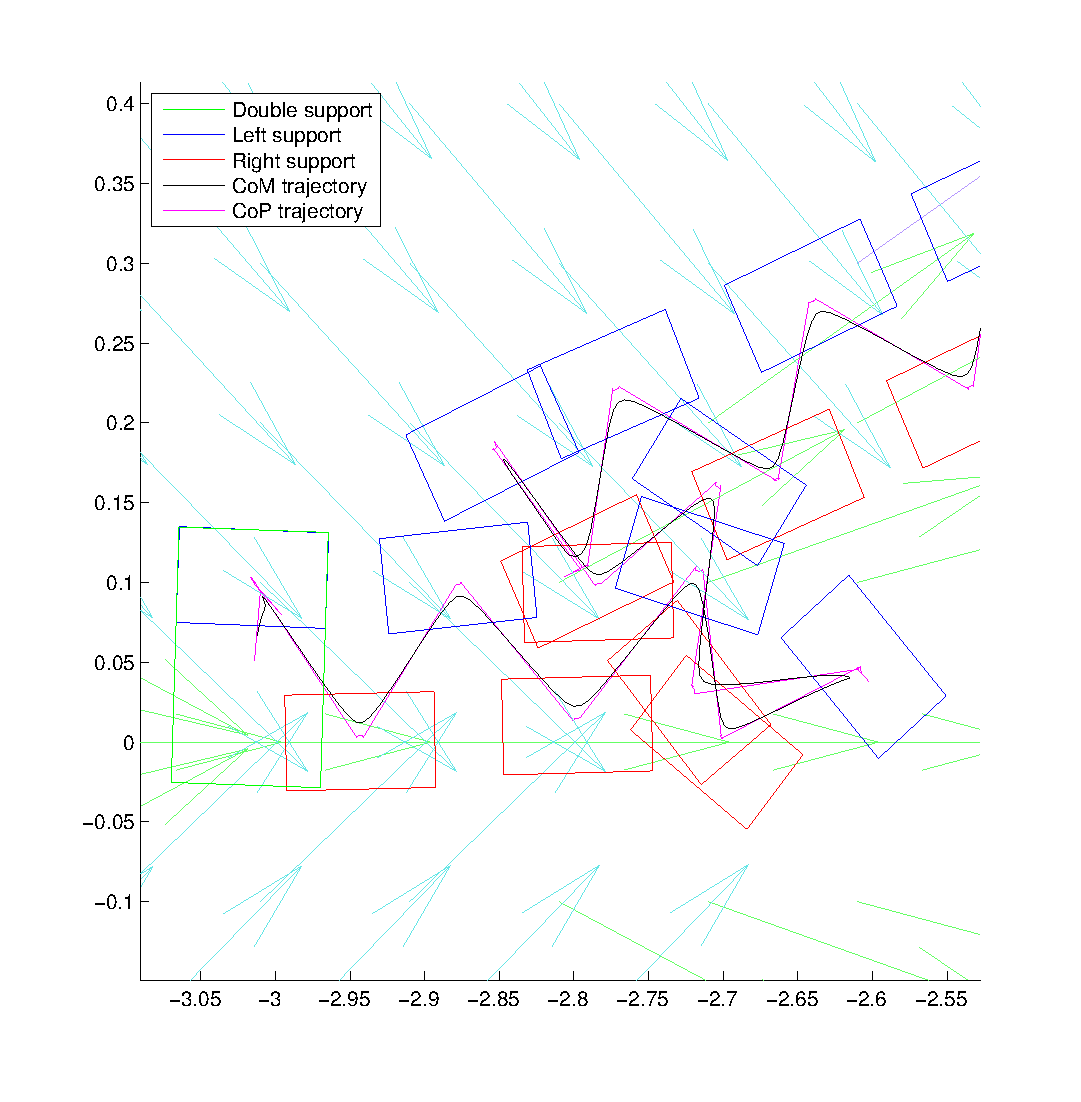
\includegraphics[scale=0.35]{figures/steps10zoom.pdf}
\caption{Zoom on Fig.~\ref{fig:steps10}, close to $(-3,0)$. As the robot compensates sliding and localization errors non-holonomically, more in-site rotations occur.}
\label{fig:steps10zoom}
\end{figure}

\begin{figure}[ht]
\centering
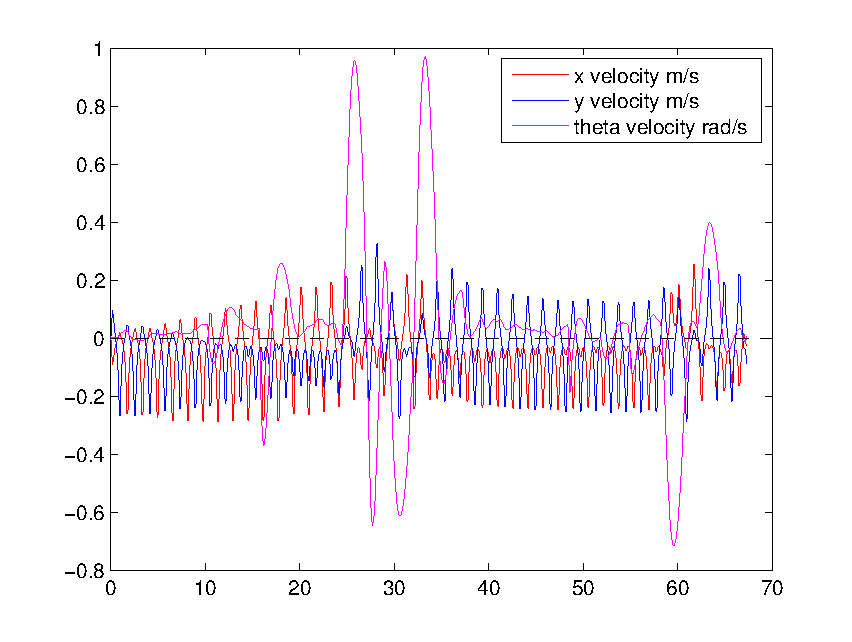
\includegraphics[scale=0.425]{figures/velocities10.pdf}
\caption{Velocities profile for the trajectory depicted in Fig.~\ref{fig:steps10}. The overshoots in the angular velocity are caused by the in-site rotations at the border of the dark blue region of the partition.}
\label{fig:velocities10}
\end{figure}

To address the aforementioned problem, we present the results of the improvement introduced in Section~\ref{sec:includingholonomic}. In Fig.~\ref{fig:steps11}, we perform the same trajectory but by introducing the possibility of holonomic motion in the region where in-site rotations would be necessary. The robot is not performing in-site rotations anymore, but a mixture of holonomic and non-holonomic motions, depending on its position with respect to the border. We can appreciate better the transition between non-holonomic and holonomic motions in Fig. \ref{fig:steps11zoom}. %Finally in Fig. \ref{fig:velocities11} we can see the reduction of the angular velocity necesay to perform the motion.

\begin{figure}[ht]
\centering
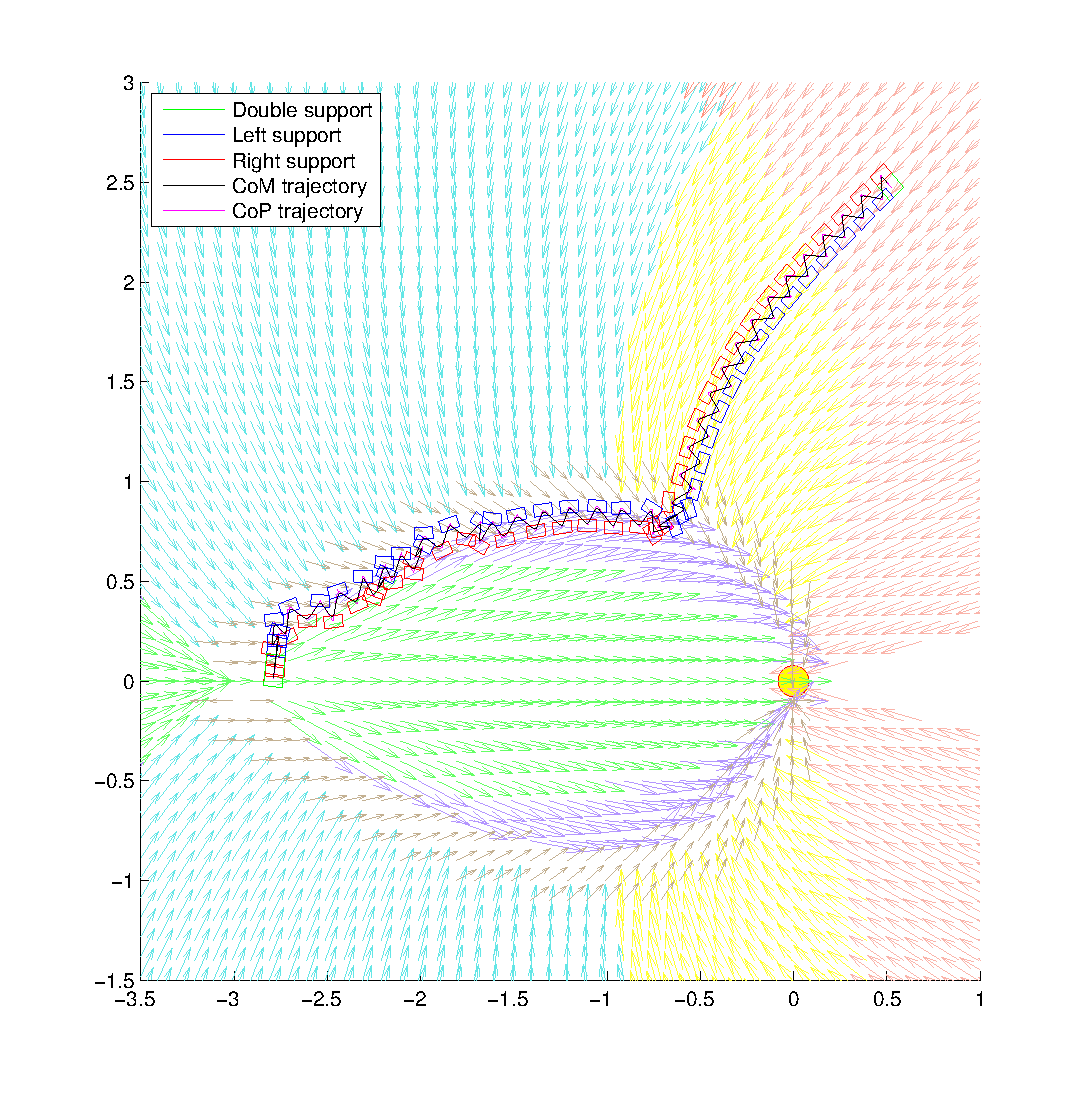
\includegraphics[scale=0.425]{figures/steps11.pdf}
\caption{Trajectory with holonomic motion made possible. Lateral motion is allowed in the khaki vector field in the orientation discontinuity region.}
\label{fig:steps11}
\end{figure}

\begin{figure}[ht]
\centering
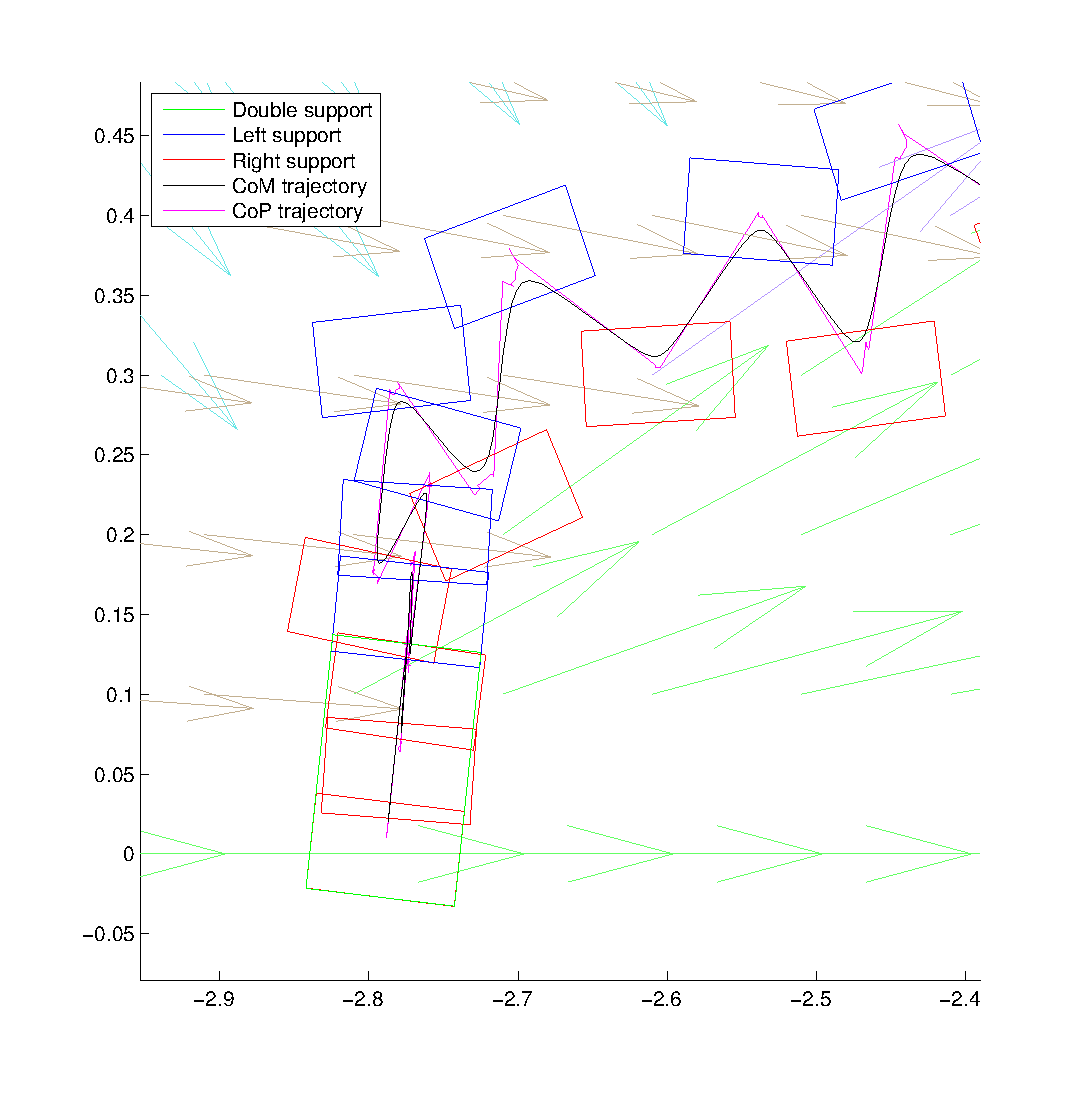
\includegraphics[scale=0.35]{figures/steps11zoom.pdf}
\caption{Transition between non-holonomic and holonomic controls. Moving sideways is much more efficient for such a trajectory to the goal.}
\label{fig:steps11zoom}
\end{figure}

%\begin{figure}
%\centering
%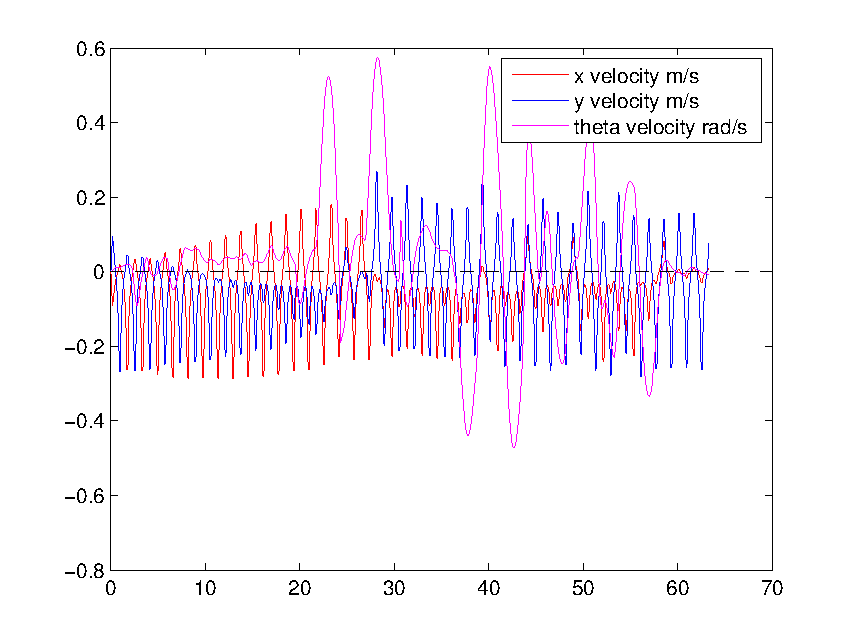
\includegraphics[scale=0.4]{velocities11.pdf}
%\caption{Velocities profile for the trajectory of the figure \ref{fig:steps11}. We can see that those velocities are in good limits and provide a stable walking. }
%\label{fig:velocities11}
%\end{figure}

%=============================================================================================================================================================
\section{Conclusion}
\label{sec:conclusion}
%=============================================================================================================================================================

In most of the current literature, the link between planning and locomotion control has been given by footsteps. In this paper, we propose a novel approach that uses directly the optimal motion synthesis derived from the planner to the control system without going through footsteps but instead by computing them within the Walking Pattern Generator. With this approach, we can drive the robot to a desired goal by using an external planner, not necessarily the one used in this paper. We tested our approach simulating real situations such a localization noise. We have also tried to make the walking pattern more efficient by introducing the possibility of using holonomic motion. Our next objective is to test the approach introduced in this paper on the HRP-2 platform.


% 3D reconstruction
\chapter{3D reconstruction} 
\label{Chap:3DReconstruction}

\subsection{Stereo-Reconstruction of Dense Surfaces}
% ~~~~~~~~~~~~~~~~~~~~~~~~~~~~~~~~~~~~~~~~~~~~~~~~~~~~~~~~~~~~~~~~~~~~~~~~~~~~~

To perform the dense reconstruction of the floor surface in front of the robot, we rely on a real-time approach similar to KinectFusion algorithm proposed in~\cite{Newcombe2011}. This approach, originally developed for a RGB-D sensor, models 3-D surfaces as zero-valued level sets of functions defined over the workspace volume. These functions are referred to as truncated signed distance function (TSDF) and they are built incrementally, by integrating the depth measurements the sensor provides, frame after frame. TSDF are defined in the 3D space, and their value is the signed distance to the closest obstacle. Here, we extend this approach, initially proposed for RGB-D depth data, to disparity data generated from a stereo head. Although the stereo data is noisier than the one from RGB-D sensors, it is a passive sensor and can be used outdoors in sunlight conditions.


Consider, as in the previous sections, that $k$ is a discretized time index. The idea is to update a mathematical representation of the surface through a volumetric TSDF model (defined over a 3D grid), referred to as $F_k$. The basic steps for integrating one new set of disparity measurements at time $k$, to update $F_k$ and the corresponding surface, are the following ones: (i) Filter the raw depth measurements generated from the stereo head, $D_k$; here we used bilateral filtering for that purpose; (ii) From these filtered measurements and the prediction of the estimated surface at the previous step, estimate the transformation between the measured surface and the predicted one using the iterative closest point algorithm (ICP) and update the camera pose; (iii) Compute a volumetric grid formed from ``local'' TSDF values $F_{D_k}$, to which confidence weights $W_{D_k}$ are associated, and integrate them into the global volumetric grid $\{F_k,W_k\}$; (iv) Predict a new surface for the next iteration by using ray-casting over the zero-crossings of the fused global volumetric grid $\{F_k,W_k\}$. 

The core of this algorithm is the computation and fusion of volumetric grids (i.e., the third step mentioned above). For a 3D point $\mathbf{p}$ expressed in the global frame $g$, its value in the current local volumetric grid $\{F_{D_k},W_{D_k}\}$ is computed as

$$
\left\{
\begin{array}{ccc}
F_{D_{k}}(\mathbf{p}) &=& \Psi (\lambda^{-1} \left \| \mathbf{t}_{g,k} - \mathbf{p}\right \| - D_k(\mathbf{x})), \\
W_{D_{k}}(\mathbf{p}) &\propto& \cos(\theta)/D_{k}(\mathbf{x}),
\end{array}
\right.
$$

with
$$
\Psi (\eta) =
\left \{
\begin{array}{cc}
\min(1,\frac{\eta}{\mu}) ~\text{sgn}(\eta) & \text{iff} ~ \eta \geq -\mu \\
\mbox{ null } & \mbox{ otherwise }
\end{array}
\right. , ~
\lambda = \left \| \mathbf{K}^{-1} [\mathbf{x}^\top 1]^\top \right \|,~
%\lambda = \left \| \mathbf{K}^{-1} \left[ \begin{matrix} \mathbf{x} \\ 1 \end{matrix} \right] \right \|,
$$

$\mu$ being a truncation distance (parameter of the algorithm), $\mathbf{x} = \pi([\mathbf{K},\mathbf 1] T^{-1}_{g,k} \mathbf{p}) \in \mathbb{R}^2$ being the image projection of $\mathbf p$. $\mathbf{K}$ is the $3\times 3$ matrix of intrinsic parameters of the camera, $\pi$ is the projection operator, $T_{g,k} = \left[ \begin{matrix} \mathbf{R}_{g,k} & \mathbf{t}_{g,k} \\ 0 & 1 \end{matrix} \right]$ the pose of the camera, at time $k$, in the global frame $g$, and $\theta$ the angle between the associated pixel ray direction and the surface normal.

The global volumetric grid at time $k$ is formed by the weighted average of all individual volumetric grids up to $k-1$. It can be shown that the optimal grid can be obtained incrementally using a simple point-wise on-line weighted average,

\begin{eqnarray*}
 F_k(\mathbf{p}) &=& \frac{W_{k-1}(\mathbf{p}) F_{k-1}(\mathbf{p}) + W_{D_{k}}(\mathbf{p}) F_{D_{k}}(\mathbf{p}) }{ W_{k-1}(\mathbf{p}) + W_{D_{k}}(\mathbf{p}) }, \\
 W_k(\mathbf{p}) &=& W_{k-1}(\mathbf{p}) + W_{D_{k}}(\mathbf{p}).
\end{eqnarray*}


To use this algorithm with stereo data and generate local data $D_k$, a disparity map from a pair of rectified images is estimated, from which the depth map $D_k$ is derived, supposing the stereo rig is completely calibrated. The literature of algorithms that estimate disparity maps is huge, but since a real time one is needed for this application, the one proposed in~\cite{Geiger2010} has been used. This algorithm estimates a piece-wise disparity map using an initial sparse disparity map of high textured points as vertices that define a triangulation of the image. Then, the dense disparity map of each sub-region is estimated by using the initial, sparse disparity map as a prior in a probabilistic scheme. The steps of the reconstruction process are illustrated in Fig.~\ref{Fig:Reconstruction}.

\begin{figure}[h]
\centering
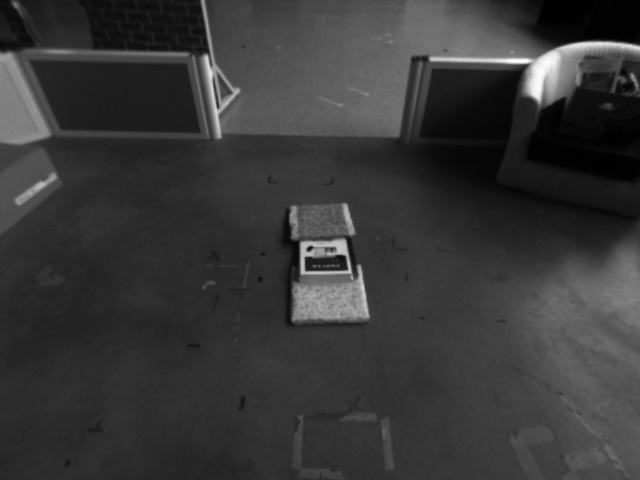
\includegraphics[scale=0.17]{figures/right0001}
\hspace{0.2cm}
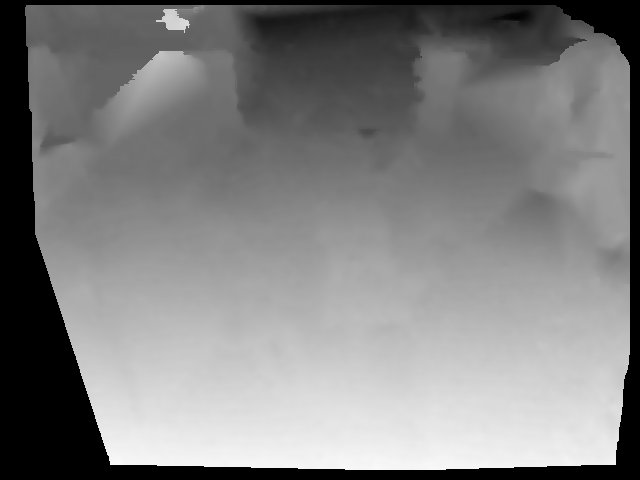
\includegraphics[scale=0.17]{figures/left0001_disp}
\hspace{0.2cm}
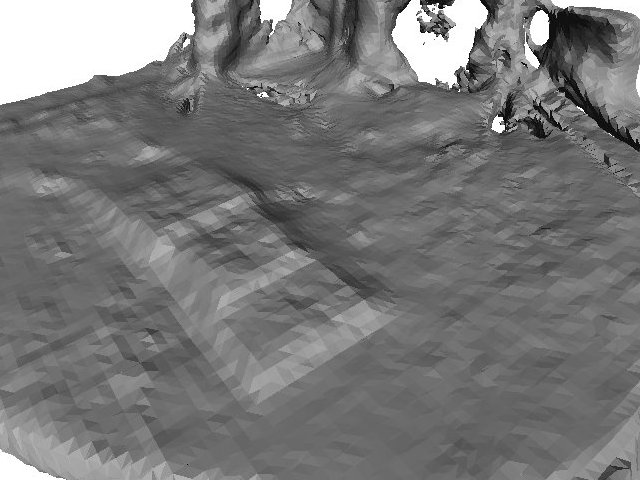
\includegraphics[scale=0.22]{figures/snapshot02}
\caption[]{From a pair of images of the scene in front of the robot (left) we estimate a dense disparity map (middle) and from this disparity map we estimate a dense surface integrating the previous frames into the volumetric grid.}
\label{Fig:Reconstruction}
\end{figure}


% Conclusions and Future Work
\begin{savequote}[10cm]
{\it ``You just can't differentiate between a robot and the very best of humans.''}
\qauthor{Isaac Asimov}
\end{savequote}

\chapter{Conclusions}
\label{Chap:Conclusions}


\bibliography{lathese}

\end{document}
